% Paquets généraux
\documentclass[a4paper,12pt,titlepage,twoside]{article}
\usepackage[T1]{fontenc}
\usepackage[utf8]{inputenc}
\usepackage[french]{babel}
\usepackage{subcaption}
\addto\captionsfrench{%
  \renewcommand{\tablename}{Tableau}%
}
\usepackage[gen]{eurosym}
%\usepackage[dvips]{graphicx}
\usepackage{minted}
\usepackage{fancyhdr}
\usepackage{pdfpages} 
\usepackage{multido}
\usepackage{hyperref}
\usepackage{textcomp}
\usepackage{schemabloc}
%\usepackage[bitstream-charter]{mathdesign}
\usepackage{array}
\newcolumntype{P}[1]{>{\centering\arraybackslash}p{#1}}
\usepackage[shortlabels]{enumitem}
\usepackage[framemethod=TikZ]{mdframed}
\usepackage{algpseudocode}
\usepackage{algorithm}

\newcommand{\nom}{Citroën AMI}
\newcommand{\numero}{08}
\newcommand{\sujet}{Citroën AMI}
\newcommand{\jour}{Jeudi 04 juin 2026}
\newcommand{\auteurun}{Renaud Costadoat}
\newcommand{\auteurdeux}{Françoise Puig}

%\usepackage{style}
\usepackage{bodegraph}
%\usepackage{rpcinematik}
\usepackage[locale = FR]{siunitx}
\usepackage{caption}
\newcommand{\institute}{Lycée Dorian}
\usepackage{calc}

\usepackage{listings}
\usepackage{fancyvrb}
\usepackage{color}
\usepackage{xcolor}
\usepackage{colortbl}
\usepackage{helvet}
\usepackage[frenchmath]{newtxsf} % for sans serif symbols
\renewcommand{\familydefault}{\sfdefault}
%\usepackage{amsfonts}
%\usepackage{amsmath}
%\usepackage{lmodern}
\usepackage{mathastext}
%\usepackage{xspace}
\usepackage{varioref}
\usepackage{tabularx}
%\usepackage{floatflt}
\usepackage{graphics}
\usepackage{wrapfig}
\usepackage{textcomp}
\usepackage{tikz,tkz-tab}
\usepackage[european resistor, european voltage, european current]{circuitikz}
\usepackage{wrapfig}
\usepackage{gensymb}
\usepackage[percent]{overpic}
\usetikzlibrary{babel}
\usepackage{ifthen}
\usepackage{cancel}
\usepackage{etoolbox}
\usepackage{multirow}
%\usepackage{boxedminipage}
\definecolor{gris25}{gray}{0.75}
\definecolor{bleu}{RGB}{18,33,98}
\definecolor{bleuf}{RGB}{42,94,171}
\definecolor{bleuc}{RGB}{231,239,247}
\definecolor{bleum}{RGB}{160,195,226}
\definecolor{rougef}{RGB}{185,18,27}
\definecolor{rougec}{RGB}{255,188,204}%255,230,231
\definecolor{vertf}{RGB}{103,126,82}
\definecolor{vertc}{RGB}{220,255,191}
\definecolor{forestgreen}{rgb}{0.13,0.54,0.13}
\definecolor{blcr}{rgb}{0.59,0.69,0.84}
\definecolor{blfr}{rgb}{0.32,0.51,0.75}
\definecolor{orfr}{rgb}{0.90,0.42,0.15}
\definecolor{orcr}{rgb}{0.90,0.65,0.50}
\definecolor{orangef}{rgb}{0.659,0.269,0.072}
\definecolor{orange}{rgb}{0.58,0.35,0.063}
\definecolor{orangec}{rgb}{0.43,0.32,0.25}
\definecolor{rcorrect}{rgb}{0.6,0,0}
\definecolor{sequence}{rgb}{0.75,0.75,0.75}
\definecolor{competences}{rgb}{0.61,0.73,0.35}
\definecolor{rose}{HTML}{ff00ff}
\definecolor{grisf}{HTML}{222222}
\definecolor{grisc}{HTML}{636363}
\definecolor{normal}{HTML}{4087c4}
\definecolor{info}{HTML}{5bc0de}
\definecolor{success}{RGB}{92,184,92}
\definecolor{warning}{RGB}{240,173,78}
\definecolor{danger}{RGB}{217,83,79}
\hypersetup{                    % parametrage des hyperliens
    colorlinks=true,                % colorise les liens
    breaklinks=true,                % permet les retours à la ligne pour les liens trop longs
    urlcolor= blfr,                 % couleur des hyperliens
    linkcolor= orange,                % couleur des liens internes aux documents (index, figures, tableaux, equations,...)
    citecolor= forestgreen                % couleur des liens vers les references bibliographiques
    }

\newcolumntype{M}[1]{>{\centering\arraybackslash}m{#1}}
\definecolor{codegreen}{rgb}{0,0.6,0}
\definecolor{codegray}{rgb}{0.5,0.5,0.5}
\definecolor{codepurple}{rgb}{0.58,0,0.82}
\definecolor{backcolour}{rgb}{0.95,0.95,0.92}

\lstdefinestyle{mystyle}{
    backgroundcolor=\color{backcolour},   
    commentstyle=\color{codegreen},
    keywordstyle=\color{magenta},
    numberstyle=\tiny\color{codegray},
    stringstyle=\color{codepurple},
    basicstyle=\ttfamily\footnotesize,
    breakatwhitespace=false,         
    breaklines=true,                 
    captionpos=b,                    
    keepspaces=true,                 
    numbers=left,                    
    numbersep=5pt,                  
    showspaces=false,                
    showstringspaces=false,
    showtabs=false,                  
    tabsize=2
}

\lstset{style=mystyle}

% Mise en page
\pagestyle{fancy}

\setlength{\hoffset}{-18pt}
\setlength{\oddsidemargin}{0pt} 	% Marge gauche sur pages impaire2s
\setlength{\evensidemargin}{0pt} 	% Marge gauche sur pages paires
\setlength{\marginparwidth}{00pt} 	% Largeur de note dans la marge
\setlength{\headwidth}{481pt} 	 	% Largeur de la zone de tête (17cm)
\setlength{\textwidth}{481pt} 	 	% Largeu\textbf{r de la zone de texte (17cm)
\setlength{\voffset}{-18pt} 		% Bon pour DOS
\setlength{\marginparsep}{7pt}	 	% Séparation de la marge
\setlength{\topmargin}{-30pt} 		% Pas de marge en haut
\setlength{\headheight}{55pt} 		% Haut de page
\setlength{\headsep}{20pt} 		% Entre le haut de page et le texte
\setlength{\footskip}{30pt} 		% Bas de\textbf{ page + séparation
\setlength{\textheight}{700pt} 		% Hauteur de l'icone zone de texte (25cm)
\setlength\fboxrule{1 pt}
\renewcommand{\baselinestretch}{1}
\setcounter{tocdepth}{1}
\newcommand{\cadre}[2]
{\fbox{
  \begin{minipage}{#1\linewidth}
   \begin{center}
    #2\\
   \end{center}
  \end{minipage}
 }
}

\newcommand{\repon}[1]
{
~\ \\
\begin{tabular}{|m{\linewidth}|}
 \hline
\multido{}{#1}{\\ \hline}
\end{tabular}
}


\newcommand{\objectif}[1]{
\mdfsetup{%
frametitle={%
\tikz[baseline=(current bounding box.east),outer sep=0pt]
\node[anchor=east,rectangle,fill=bleum]
{\strut Objectif~};}}
\mdfsetup{innertopmargin=10pt,linecolor=bleum,%
linewidth=2pt,topline=true,%
frametitleaboveskip=\dimexpr-\ht\strutbox\relax
}
\begin{mdframed}[]\relax%
#1
\end{mdframed}}


\newcounter{num_quest} \setcounter{num_quest}{0}
\newcounter{num_rep} \setcounter{num_rep}{0}
\newcounter{num_cor} \setcounter{num_cor}{0}

\newcommand{\feuilleDR}[1]{
	\begin{tikzpicture}
		\draw[gray!30](0,0)grid[step=0.5cm](\linewidth,#1);
	\end{tikzpicture}
}

%\newcommand{\question}[1]{\refstepcounter{num_quest}\par
%~\ \\ \parbox[t][][t]{0.15\linewidth}{\textbf{Question \arabic{num_quest}}}\parbox[t][][t]{0.85\linewidth}{#1\label{q\the\value{num_quest}}}\par
%}

\newcommand{\question}[1]{\refstepcounter{num_quest}\par
~\ \\ \textbf{Question \arabic{num_quest} : }#1\label{q\the\value{num_quest}}\par
}

\newcommand{\posetafigure}[3]{
\begin{figure}[ht!]
 \begin{center}
  \includegraphics[width=#2\linewidth]{img/#1}
 \end{center}
 \caption{\label{#1} #3}
\end{figure}}

\newcommand{\goforum}{
\begin{figure}

\end{figure}
\begin{center}
 
\includegraphics[width=0.7\linewidth]{../../../img/go_forum}
\end{center}
\label{go_forum}
\caption{J'pète les plombs}
\end{figure}}

\newcommand{\reponse}[4][1]
{\noindent
\parbox{\textwidth}{
\rule{\linewidth}{.5pt}\\
\textbf{Question\ifthenelse{#1>1}{s}{} \multido{}{#1}{%
\refstepcounter{num_rep}\ref{q\the\value{num_rep}} }:} ~\ \\
\ifdef{\public}{#3 \ifthenelse{#2>0}{~\ \\ 	\feuilleDR{#2}}}{#4}
}}

\NewDocumentEnvironment{reponseminted}{O{1} m m +b}{%
% ======== BEGIN ========
\noindent
\begin{minipage}{\textwidth}
\rule{\linewidth}{.5pt}\\
\textbf{Question%
\ifthenelse{#1>1}{s}{}%
\multido{}{#1}{\refstepcounter{num_rep}\ref{q\the\value{num_rep}}}:}%
\\[0.4em]

\ifdef{\public}{%
    #3%
    \ifthenelse{#2>0}{\\[0.5em]\feuilleDR{#2}}{}%
}{}

\end{minipage}

% ======== END OF MINIPAGE ========

\ifdef{\public}{}{% si pas public, afficher le corrigé verbatim
#4%
}
}



\newboolean{printdr}
\newboolean{printcor}
\setboolean{printdr}{false}
\setboolean{printcor}{false}

\newcommand{\reponseinfo}[2][1]
{\noindent
\rule{\linewidth}{.5pt}\\
\textbf{Question\ifthenelse{#1>1}{s}{} \multido{}{#1}{%
\refstepcounter{num_rep}\ref{q\the\value{num_rep}} }:} ~\ \\
\ifdef{\public}{\parbox{\textwidth}{\ifthenelse{#2>0}{~\ \\ 	\feuilleDR{#2}}}
\setboolean{printdr}{true}\setboolean{printcor}{false}}
{\setboolean{printdr}{false}\setboolean{printcor}{true}}
}

\newcommand\sautpage[1]{
\ifdef{\public}{\multido{}{#1}{~\ \newpage}}
}


\makeatletter
\newcommand\modulo[2]{
    \newcounter{lastpagesujet}
	\setcounter{lastpagesujet}{#1}
    \divide\value{lastpagesujet} by #2
    \multiply\value{lastpagesujet} by #2
    \advance\value{lastpagesujet} by #2
    \advance\value{lastpagesujet} by 1\relax
    }
\makeatother

\newcommand{\finsujet}[1]
{
    \begin{center}
    \Large{FIN}
    \end{center}
        
    \ifthenelse{\equal{#1}{public}}{\def\public{}}{}

}

\newcommand{\debutcor}
{	
    \ifdef{\public}{
        \pagestyle{docreponse}
	}{\pagestyle{correction}}


    \ifdef{\public}{
    \begin{center}
        \begin{tikzpicture} 
            \draw (0,0) rectangle (2,2);
            \draw (0,0) -- (2,2);
            \draw (1.5,0.5) node {\large 20};
            \draw (2,0) rectangle (17,2);
            \draw (4,1.7) node {\large Commentaires:};
            \draw (0,2) rectangle (8.5,3);
            \draw (8.5,2) rectangle (17,3);
            \draw (1,2.5) node {\large NOM:};
            \draw (9.7,2.5) node {\large Prénom:};
        \end{tikzpicture}
    \end{center}
    }
}

\newcommand{\ecrirenom}
{	

    \ifdef{\public}{
    \newpage
    
    \begin{center}
        \begin{tikzpicture} 
            \draw (0,0) rectangle (8.5,1);
            \draw (8.5,0) rectangle (17,1);
            \draw (1,0.5) node {\large NOM:};
            \draw (9.7,0.5) node {\large Prénom:};
        \end{tikzpicture}
    \end{center}
    
    }
}

%\newcommand{\repcarre}[2]
%{
%~\ \\
%\begin{tikzpicture}
%\draw [fill=white] (0,0) rectangle +(\linewidth,#1);
%\node[align=left] at (1.1,#2-0.3) {\textbf{Question #1:}};
%\end{tikzpicture}
%}

\newcommand{\titre}[1]
{\begin{center}
\cadre{0.8}{\huge #1} 
\end{center}
}


%Définition des torseurs :
\newcommand{\torseur}[2]{\left\{\mathcal{#1}_{#2} \right\}}
\newcommand{\torseurh}[3]{\left\{\genfrac{}{}{0pt}{0}{#1}{#2}\right\}_{#3}}
\newcommand{\torseurv}[8]{\left\{
\begin{matrix}
#1 & #4 \\ #2 & #5 \\ #3 &#6
\end{matrix}
\right\}_{{#7},{#8}}}

%Définition des torseurs :
%\newcommand{\torseur}[2]{\left \{\mbox{\relsize{2}{$\mathcal {#1}$}\relsize{-2}}\phantom{}_{\mbox{\scriptsize $#2$}} \right \}}
%\newcommand{\torseurh}[3]{\left\{\genfrac{}{}{0pt}{0}{#1}{#2}\right\}_{#3}}
%\newcommand{\torseurv}[8]{
%\left\{\begin{array}{@{}c|c@{}} #1 & #4 \\ #2 & #5 \\ #3 & #6 \end{array} \right\}_{#7,#8}
%}
\newcommand{\derivee}[2]{\left.\dfrac{\d #1}{\d t}\right|_{#2}}
\newcommand{\tripleint}{\int\!\!\!\!\!\int\!\!\!\!\!\int}

% Notation cinématique et statique
\newcommand{\cinematique}[2]{\mbox{#1}/\mbox{#2}}
\newcommand{\statique}[2]{\mbox{#1}\rightarrow\mbox{#2}}
\newcommand{\moment}[3]{\vv {#1}_{\scriptsize{#3}}(#2)}
\newcommand{\resultante}[2]{\vv {#1}_{\scriptsize{#2}}}


%Commande de base
\newcommand{\jo}{\left(j\omega\right)} % j \omega dans l'analyse fréquentielle
\newcommand{\tl}{\xrightarrow{\mathcal{L}}} % transformée de laplace sur fleche
\newcommand{\tli}{\xrightarrow{\mathcal{L}^{-1}}} % transformée inverse de laplace sur fleche
\renewcommand{\d}[1][]{\mathrm{d#1}}
\newcommand{\dd}[1][]{\mathrm{d#1}}
\newcommand{\vect}[2]{{#1}\wedge{#2}}
\newcommand{\base}[3]{(\vec #1,\vec #2,\vec #3)}
\newcommand{\vectbase}[4]{{\vphantom{\left| \begin{matrix}
#1\\#2\\#3 \end{matrix} \right|}}_{#4}{\left| \begin{matrix}
#1\\#2\\#3 \end{matrix} \right.}}
%Pour avoir les paragraphes sous la forme I, II, III
\renewcommand{\thesection}{\Roman{section}}
\setcounter{secnumdepth}{3}
\renewcommand{\Frlabelitemii}{$\bullet$}

% En tête et pied de page
\lhead{\nom}
\rhead{
\includegraphics[width=2cm]{../../../img/logo}}
\lfoot{\auteurun,\ \auteurdeux}
\cfoot{Page \thepage}

\fancypagestyle{docreponse}{%
  \fancyhf{}
%  \fancyhead[LO]{NOM Prénom: .............................}
  \rhead{
\includegraphics[width=2cm]{../../../img/logo}\hspace{2pt}}
  \ifdef{\auteurdeux}{\lfoot{\auteurun,\ \auteurdeux}}{\lfoot{\auteurun}}
  \rfoot{\sujet}
  \lfoot{Document réponse}
  \cfoot{Page \thepage}
   }

\fancypagestyle{correction}{%
  \fancyhf{}
  \lhead{\colorbox{danger}{\begin{minipage}{0.65\paperwidth} \textcolor{white}{\textbf{Correction}} \end{minipage}} }
  \rhead{
\includegraphics[width=2cm]{../../../img/logo}}
  \lfoot{Renaud Costadoat, Françoise Puig}
  \rfoot{\colorbox{danger}{\begin{minipage}{0.3\paperwidth} \begin{flushright}\textcolor{white}{\textbf{Correction}}\end{flushright} \end{minipage}} }
  \cfoot{Page \thepage}
}

\fancypagestyle{correctioninfo}{%
  \fancyhf{}
  \lhead{\colorbox{danger}{\begin{minipage}{0.65\paperwidth} \textcolor{white}{\textbf{Correction}} \end{minipage}} }
  \rhead{
\includegraphics[width=2cm]{../../../img/logo}}
  \lfoot{Renaud Costadoat, Juliette Genzmer}
  \rfoot{\colorbox{danger}{\begin{minipage}{0.6\paperwidth} \begin{flushright}\textcolor{white}{\textbf{Correction}}\end{flushright} \end{minipage}} }}

\renewcommand{\footrulewidth}{0.4pt}

\usepackage{eso-pic}
\newcommand{\BackgroundPic}{%
\put(0,0){%
\parbox[b][\paperheight]{\paperwidth}{%
\vfill
\begin{center}
\hspace{0.5cm}\vspace{0.5cm}

\includegraphics[width=\paperwidth,height=\paperheight,%
keepaspectratio]{../../../img/fond3}%
\end{center}
\vfill
}}}

\newcommand{\BackgroundPicdeux}{%
\put(25,-30){%
\parbox[b][\paperheight]{\paperwidth}{%
\vfill
\begin{center}
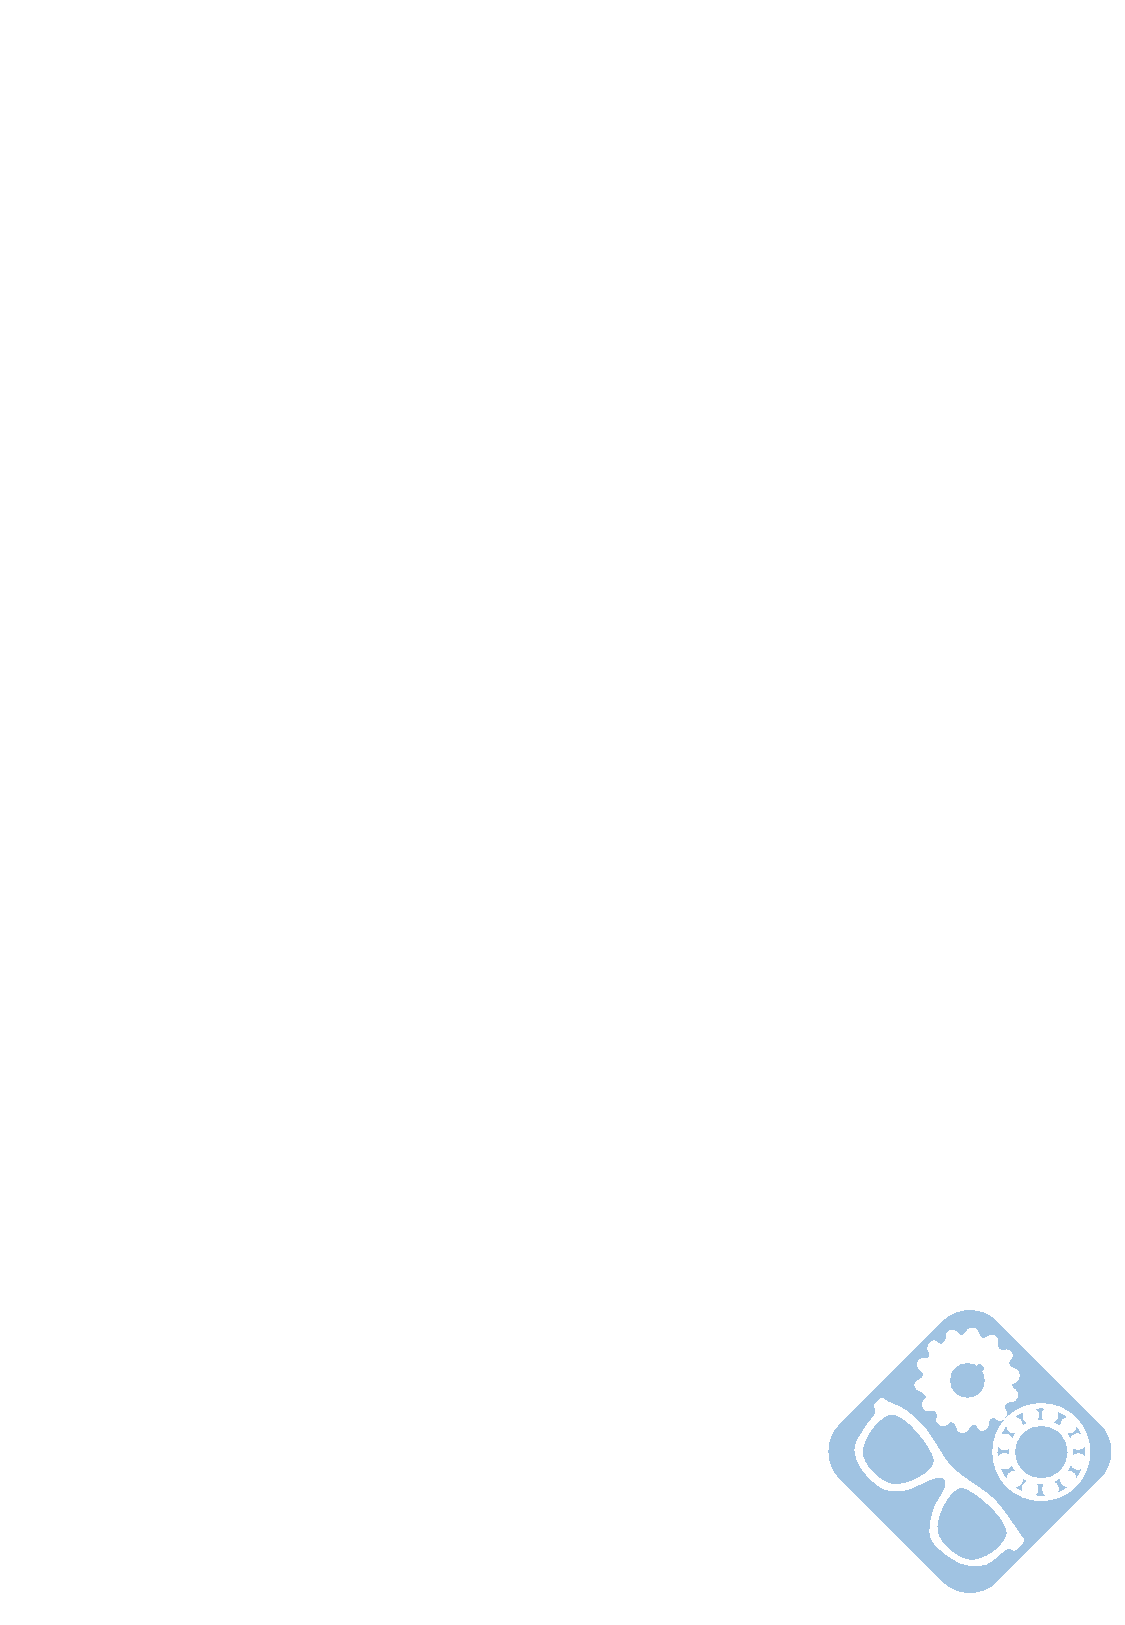
\includegraphics[width=\paperwidth,height=\paperheight,%
keepaspectratio]{../../../img/fond4}%
\end{center}
\vfill
}}}

\begin{document}

\pagestyle{empty}

\AddToShipoutPicture*{\BackgroundPic}


\includegraphics[width=2cm]{../../../img/logo}

\Huge{DS \numero - \sujet}

\vspace{1cm}

\ifdef{\prive}{\begin{center}\colorbox{danger}{\Huge{Avec Correction}}\end{center}}{}

\begin{center}
\centering\huge{PTSI}
\end{center}

\vspace{2cm}


\begin{center}
\centering\Large{\jour}
\end{center}

\vspace{2cm}

\normalsize

\tableofcontents

\newpage

\AddToShipoutPicture{\BackgroundPicdeux}

\pagestyle{fancy}

\begin{center}
\Huge \sujet
\end{center}


\normalsize


\section{Présentation du système étudié}

\begin{minipage}{0.55\linewidth}
L'AMI, figure \ref{fig01}, est une voiture sans permis 100\,\% électrique à deux places du constructeur automobile français Citroën, produite et commercialisée à partir de mai 2020.

Elle permet un déplacement urbain et écologique, puisque sans production de gaz à effet de serre (GES), pour 2 personnes. L'âge de conduite minimum est de 14 ans, l'AMI étant considérée comme un quadricycle léger à moteur.
\end{minipage}
\hfill
\begin{minipage}{0.42\linewidth}
  \centering
  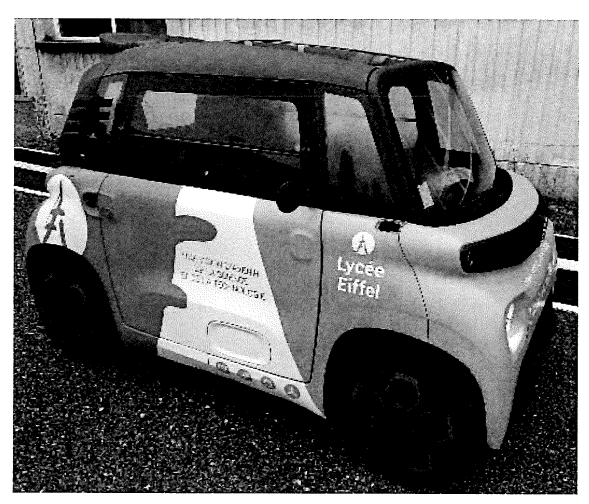
\includegraphics[width=0.9\linewidth]{img/fig01.png}
  \captionof{figure}{\label{fig01} Voiture AMI}
\end{minipage}

\vspace{0.5em}
Le fonctionnement général de la voiture est donné sur le document technique DT1. Deux diagrammes SysML sont également fournis pour décrire l'utilisation de l'AMI (figure \ref{fig02}) et définir certaines exigences (figure \ref{fig03}).


\begin{figure}[!ht]
\centering
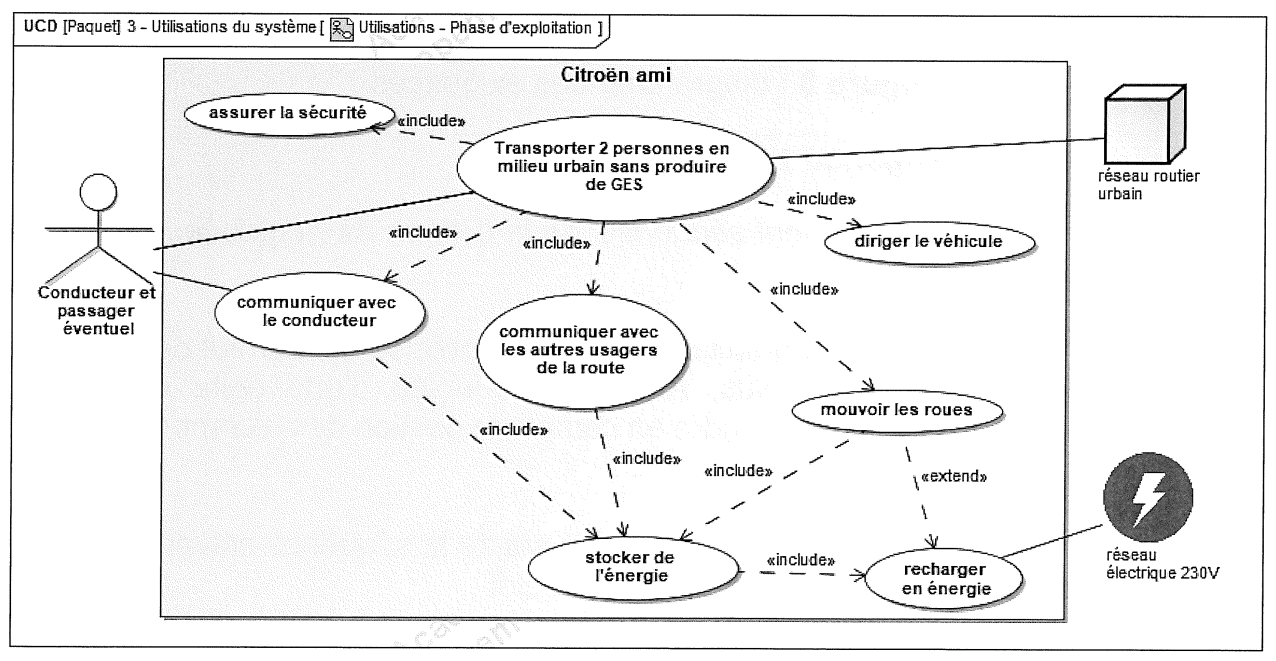
\includegraphics[width=0.85\linewidth]{img/fig02.png}
\caption{\label{fig02} Diagramme des cas d'utilisation}
\end{figure}

\newpage

\begin{figure}[!ht]
\centering
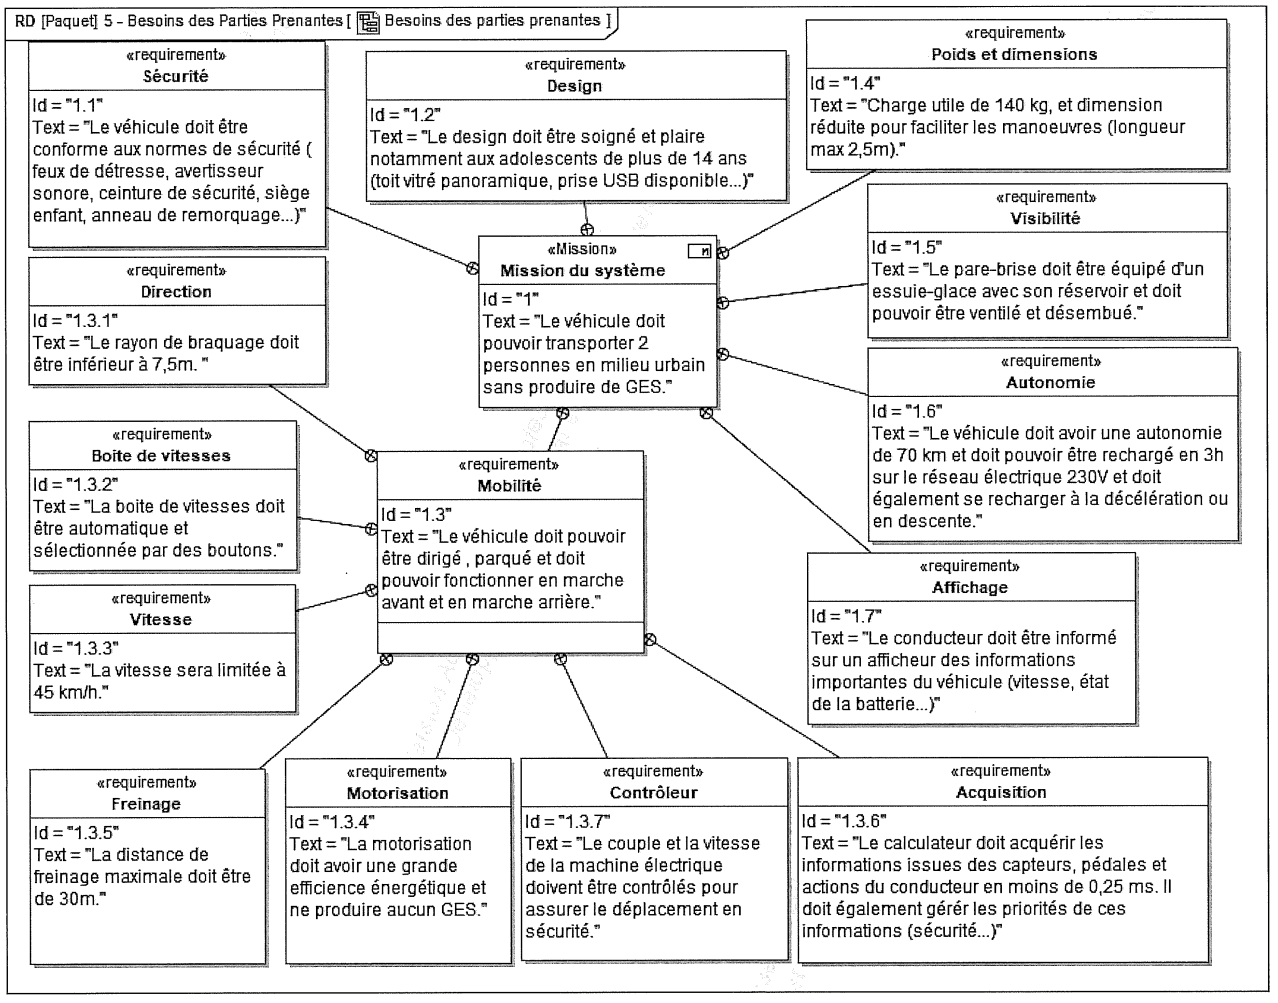
\includegraphics[width=0.85\linewidth]{img/fig03.png}
\caption{\label{fig03} Diagramme des exigences}
\end{figure}

\section{Validation de l'exigence 1.3.2}

\textbf{Objectif :} \textit{valider le fonctionnement séquentiel de la Citroën AMI équipée d'une boîte de vitesse automatique.}

La mise en route de la Citroën AMI suit une séquence précise qui permet de sécuriser le démarrage du véhicule. De plus, AMI étant équipée d'une boîte de vitesse automatique, il est nécessaire de prendre en compte la gestion de ce composant dans le programme de mise en route.

Afin de démarrer le véhicule, il est nécessaire de suivre la séquence suivante :
\begin{itemize}
  \item déverrouillage et ouverture des portes avec la clef ;
  \item déblocage du volant en tournant la clef d'un demi-tour dans le dispositif d'antivol de la colonne de direction ;
  \item mise en route de l'ordinateur de bord en tournant la clef d'un quart de tour supplémentaire ;
  \item appui sur le frein à pied ;
  \item choix de la vitesse de départ (D = marche avant, N = point mort, R = marche arrière) ;
  \item déverrouillage du frein à main ;
  \item relâchement du frein à pied ;
  \item déplacement contrôlé à l'aide de l'accélérateur.
\end{itemize}

Le diagramme d'état de la figure \ref{fig04} modélise la séquence précédente accompagnée de tous les autres éléments nécessaires à la mise en route du véhicule. Les différents voyants indiqués dans le diagramme d'états sont présents sur l'afficheur du tableau de bord de la Citroën AMI présenté en figure \ref{fig05}.

\begin{figure}[!ht]
\centering
	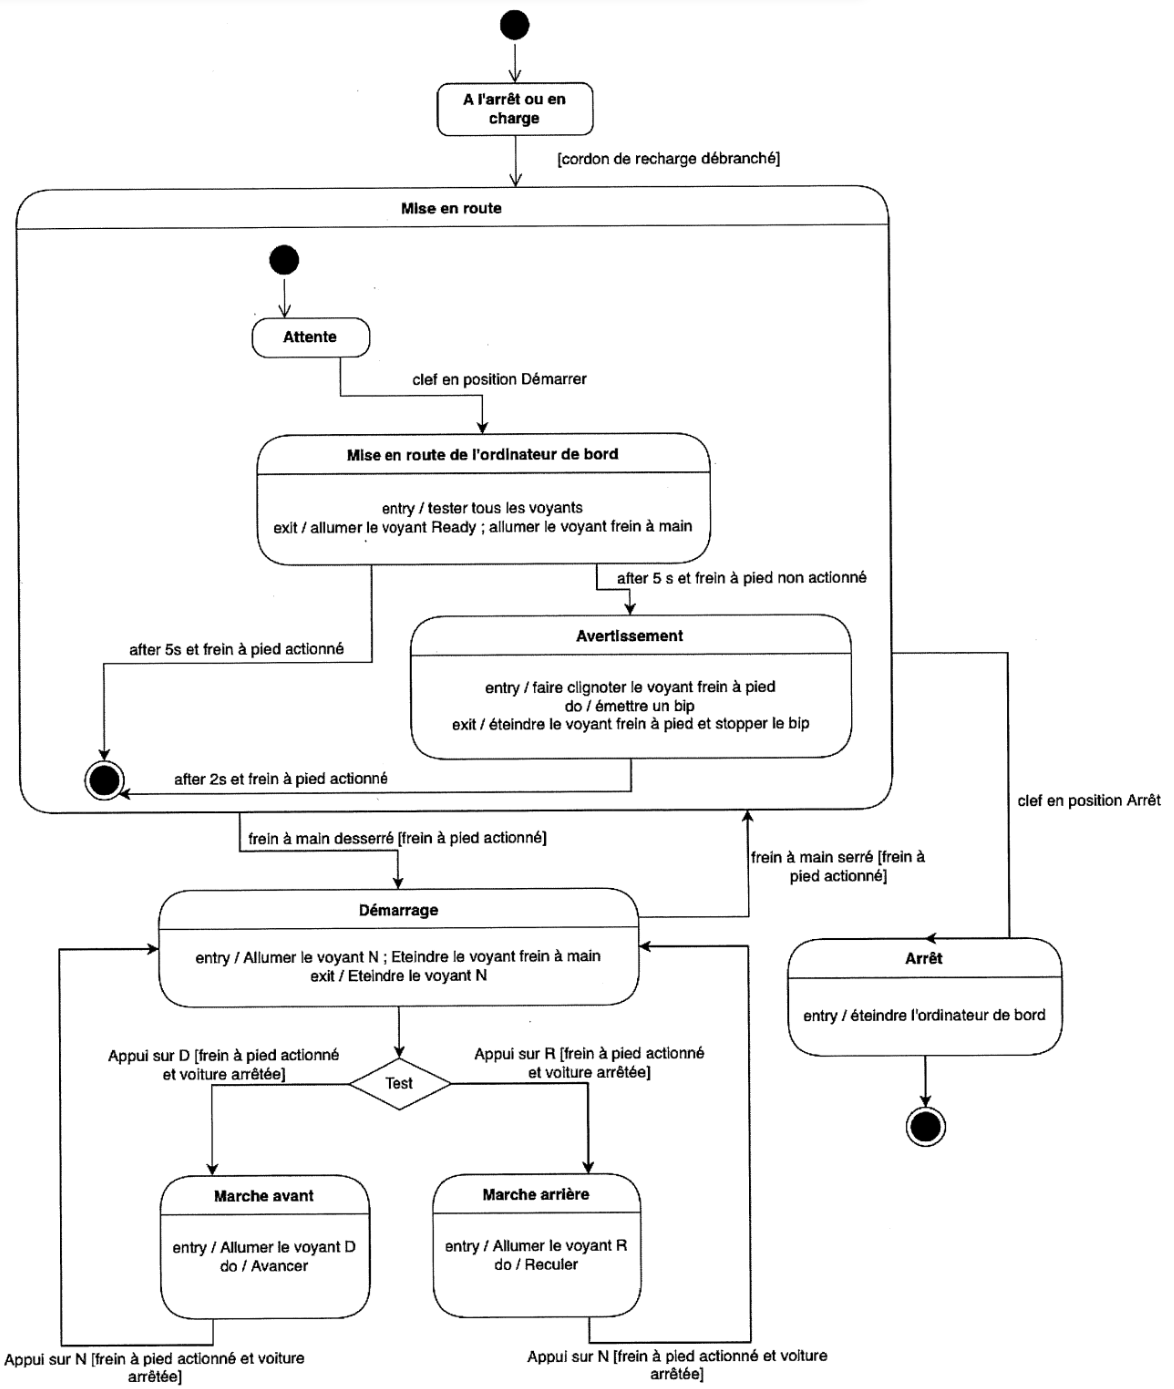
\includegraphics[width=0.82\linewidth]{img/fig04.png}
\caption{\label{fig04} Diagramme d'état de la mise en route de la Citroën AMI}
\end{figure}

\newpage

\begin{figure}[!ht]
\centering
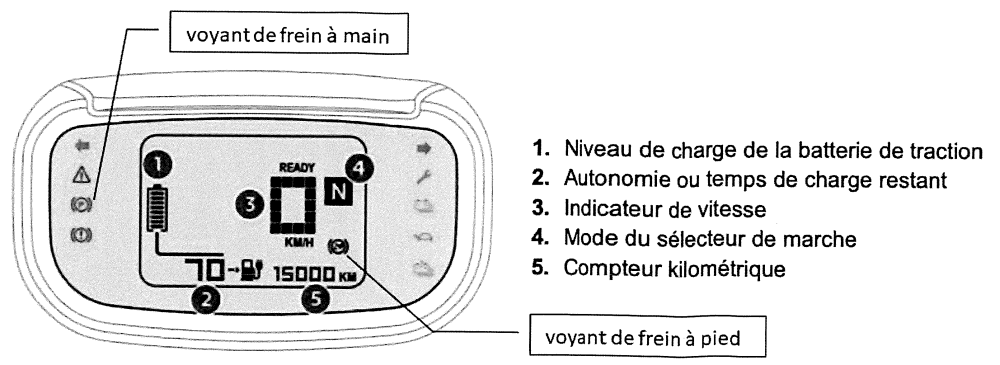
\includegraphics[width=0.6\linewidth]{img/fig05.png}
\caption{\label{fig05} Afficheur du tableau de bord de la Citroën AMI}
\end{figure}

\question{En supposant l'état « Mise en route de l'ordinateur de bord » actif initialement, compléter les chronogrammes des variables suivantes sur le document-réponse :
\begin{itemize}[noitemsep]
\item Démarrage ; \item Avertissement ; \item Émettre un bip ; \item Voyant D allumé ; \item Marche avant ; \item Voiture arrêtée.
\end{itemize}}

\section{Validation de l'exigence 1.3.1}

\textbf{Objectif :} \textit{réaliser le modèle mécanique de la direction afin de valider la valeur numérique du rayon de braquage de 7,5\,m.}

La Citroën AMI possède des caractéristiques géométriques intéressantes pour la circulation en ville. Ses faibles dimensions permettent une conduite très efficiente en circuit urbain avec un rayon de braquage très faible. Le modèle mécanique de la direction du véhicule est représenté sur le schéma cinématique de la figure \ref{fig06}.

\begin{figure}[!ht]
\centering
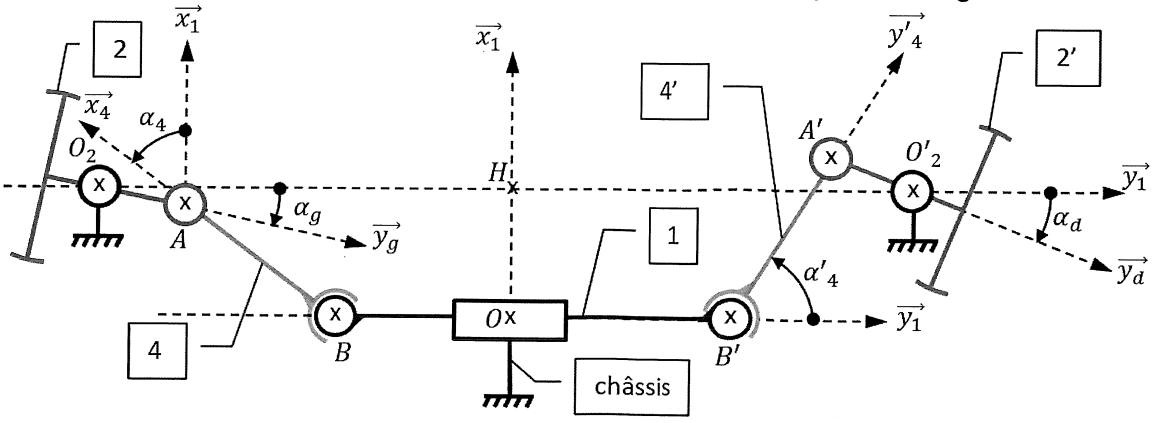
\includegraphics[width=0.85\linewidth]{img/fig06.png}
\caption{\label{fig06}Schéma cinématique de la direction}
\end{figure}

La crémaillère 1 est reliée à la colonne de direction par l'intermédiaire d'un système pignon crémaillère de rayon 15\,mm, l'amplitude de rotation du volant est de 2 tours. La crémaillère 1 est en liaison glissière de direction $\overrightarrow{y_1}$ avec le châssis du véhicule. Les biellettes de direction 4 et 4' sont en liaison sphérique de centre B (respectivement B') avec la crémaillère 1. Elles sont également en liaison pivot d'axe $(A,\overrightarrow{z_1})$ (respectivement $(A',\overrightarrow{z_1})$) avec les ensembles roue avant droite 2 et gauche 2'. Les roues avant droite 2 et gauche 2' sont en liaison pivot d'axe $(O_2,\overrightarrow{z_1})$ (respectivement $(O'_2,\overrightarrow{z_1})$) avec le châssis.

\textbf{On pose :}

\begin{center}
\renewcommand{\arraystretch}{1.5}
\begin{tabular}{|c|c|c|}
\hline
$\overrightarrow{O_2A} = a\cdot\overrightarrow{y_g}$ & $\overrightarrow{AB} = -l\cdot\overrightarrow{x_4}$ & $\overrightarrow{A'B'} = -l'\cdot\overrightarrow{y'_4}$ \\
\hline
$\overrightarrow{O'_2A'} = -a\cdot\overrightarrow{y_d}$ & $\overrightarrow{O_2O'_2} = d\cdot\overrightarrow{y_1}$ & $\overrightarrow{BB'} = L\cdot\overrightarrow{y_1}$ \\
\hline
$\overrightarrow{OB} = -y(t)\cdot\overrightarrow{y_1}$ & $\overrightarrow{OH} = e\cdot\overrightarrow{x_1}$ & $\overrightarrow{O_2H} = \dfrac{d}{2}\cdot\overrightarrow{y_1}$ \\
\hline
\end{tabular}
\end{center}

Les différentes bases liées aux solides, nécessaires aux calculs, sont repérées par les figures de changement de base de la figure \ref{fig07}.

\begin{figure}[!ht]
\centering
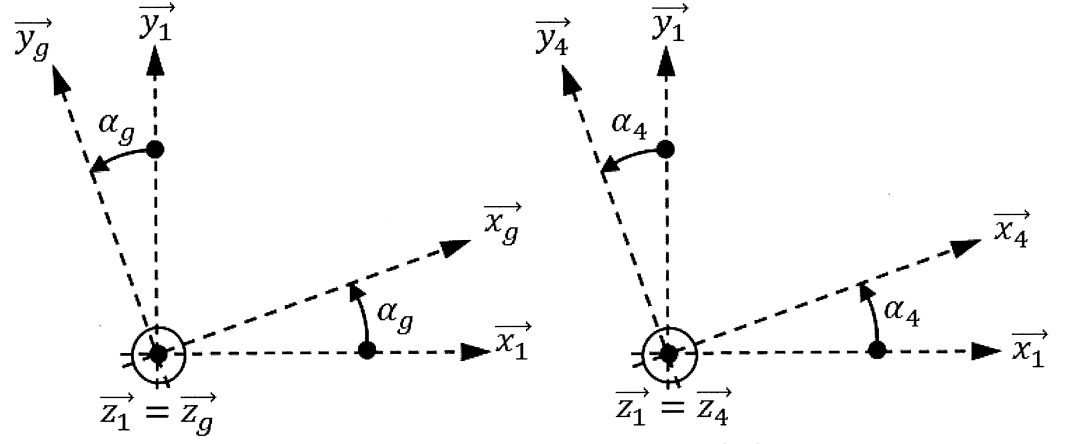
\includegraphics[width=0.7\linewidth]{img/fig07.png}
\caption{\label{fig07}Figures de changement de base}
\end{figure}

\question{Réaliser le graphe des liaisons du mécanisme de la direction représenté sur la figure \ref{fig06} en complétant le document-réponse.}

\question{Déterminer le degré d'hyperstatisme du mécanisme.}

\question{Proposer une (des) modification(s) de liaison(s) afin de rendre le modèle isostatique.}

\question{Écrire la fermeture géométrique vectorielle $\{OBAO_2HO\}$.}


\question{Projeter cette équation vectorielle dans la base $(\overrightarrow{x_1}, \overrightarrow{y_1})$ afin de déterminer deux équations scalaires reliant les données géométriques du problème.}

\question{En déduire l'expression de $y(t)$ en fonction de $\alpha_g(t)$ et des constantes du problème.}

\newpage

L'inversion de cette équation non-linéaire ne peut être facilement réalisée analytiquement. Un modèle numérique permettra de déterminer l'évolution des angles de braquage en fonction d'une rotation à gauche du volant de 1 tour à partir de la position centrale. On se propose d'utiliser un algorithme de résolution par dichotomie pour déterminer l'angle de la roue gauche $\alpha_g(t)$ en fonction du déplacement de la crémaillère $y(t)$. Le pseudo-code  du programme répondant à cette problématique est présenté sur le document technique DT3.

Nous considérerons que la position centrale du volant, et donc de la crémaillère, correspond au couple de valeurs : ($\alpha_g = 0 \degree$, $y=200mm$). La rotation du volant se fait vers la gauche, pour un tour entier. On rappelle que le rayon du pignon de la crémaillère vaut 15mm.

\question{Indiquer les valeurs de $u$ et $v$ à prendre au début de l'algorithme de dichotomie afin de déterminer $\alpha_g$ pour une rotation du volant d'un tour entier vers la gauche.}

\question{Expliquer le rôle de la variable $\varepsilon$ dans l'algorithme.}

\medskip Afin de déterminer toutes les valeurs de $\alpha_g$ lors de la rotation du volant, il faut appliquer l'algorithme de dichotomie successivement pour plusieurs valeurs de $y$ et stocker toutes les valeurs renvoyées.

\question{Indiquer les valeurs extrêmes $(y_{min},y_{max})$ à prendre pour déterminer toutes les valeurs de $\alpha_g$ lors du déplacement de la crémaillère.}

\medskip Le résultat de cette simulation numérique permet de tracer l'évolution des angles$\alpha_d$ et $\alpha_g$ en fonction du déplacement de la crémaillère $y$ représentées sur les courbes de la figure \ref{fig08}.

\begin{figure}[H]
\centering
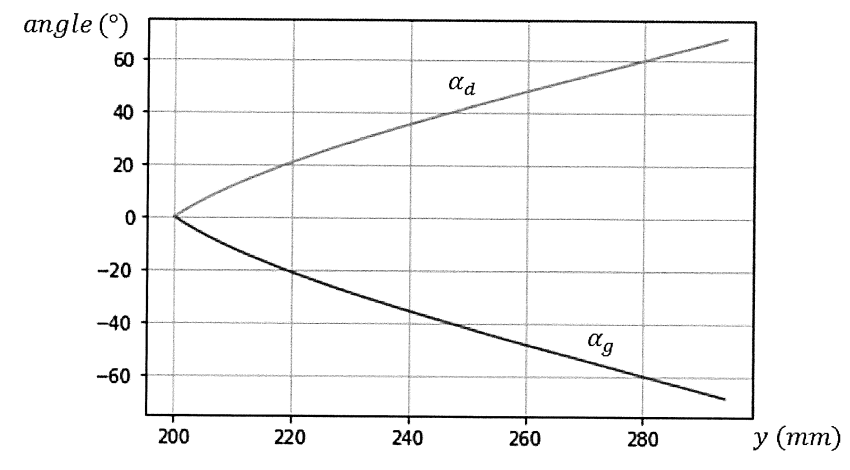
\includegraphics[width=0.7\linewidth]{img/fig08.png}
\caption{\label{fig08}Évolution des angles $\alpha_d$ et $\alpha_g$ en fonction du déplacement de la crémaillère $y$}
\end{figure}

\question{Déterminer les angles de braquage maximal des roues avant.}

\newpage

Sur la Citroën AMI, les roues avant sont directrices et motorisées. Lors d'un virage, les vitesses des roues s'adaptent automatiquement afin d'assurer en permanence le roulement sans glissement. Les roues arrières sont non motorisées et non directrices. Un différentiel mécanique permet d'assurer la compatibilité des vitesses de rotation des roues avant avec la condition de roulement sans glissement.

\medskip
Supposons une prise de virage vers la gauche du véhicule. Le modèle mécanique de cette étude de cas est représenté sur la figure \ref{fig09}.

\begin{figure}[H]
\centering
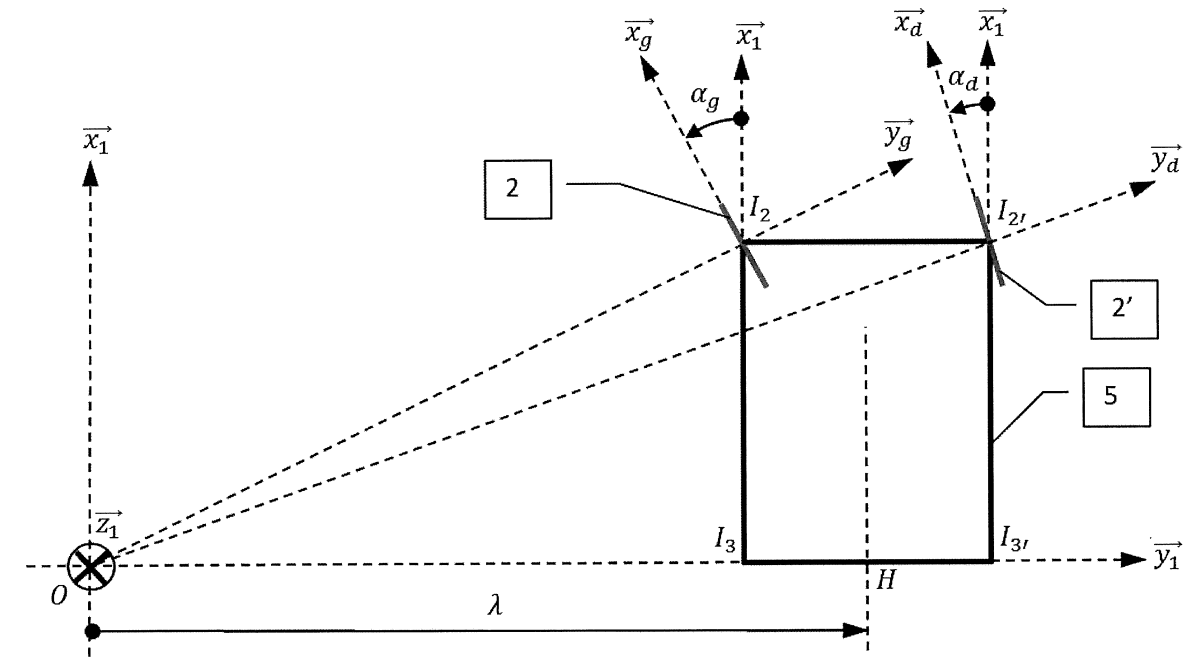
\includegraphics[width=0.82\linewidth]{img/fig09.png}
\caption{\label{fig09}Modèle mécanique pour un virage vers la gauche}
\end{figure}

Le mouvement de la roue avant gauche par rapport au châssis est modélisé par le torseur cinématique suivant :$\{V_{2/5}\} = \left\{\begin{array}{c} \omega_g\cdot\overrightarrow{y_g} \\ \overrightarrow{0} \end{array}\right\}_{O_2}$
avec $\omega_g$ vitesse angulaire de la roue gauche par rapport au châssis 5.

\medskip
Le mouvement de la roue avant droite par rapport au châssis est modélisé par le torseur cinématique suivant :$
\{V_{2'/5}\} = \left\{\begin{array}{c} \omega_d\cdot\overrightarrow{y_d} \\ \overrightarrow{0} \end{array}\right\}_{O_{2'}}$ avec $\omega_d$ vitesse angulaire de la roue droite par rapport au châssis 5.

\medskip
Le mouvement du châssis 5 du véhicule par rapport au sol 0 est représenté par le torseur cinématique suivant :$\{V_{5/0}\} = \left\{\begin{array}{c} \omega_{50}\cdot\overrightarrow{z_1} \\ \overrightarrow{0} \end{array}\right\}_{O}$ avec $\omega_{50}$ vitesse angulaire du châssis par rapport au sol.

\medskip
Il s'agit d'une rotation autour du point O. Pour assurer ce virage, le conducteur actionne la colonne direction en orientant les roues avant 2 et 2' d'un angle de braquage $\alpha_g$ et $\alpha_d$ par rapport au châssis.

\medskip
Il sera supposé dans toute cette partie que la condition de roulement sans glissement est assurée pour tous les points de contact entre les 4 roues et le sol en $I_2$, $I_{2'}$, $I_3$ et $I_{3'}$. Les centres des roues sont notés $O_2$, $O_{2'}$, $O_3$ et $O_{3'}$. Le rayon de braquage du véhicule est la longueur $\|\overrightarrow{OH}\| = \lambda$.

\textbf{On pose :}
\begin{center}
\renewcommand{\arraystretch}{1.5}
\begin{tabular}{|c|c|c|}
\hline
$\overrightarrow{I_2I_{2'}} = d\cdot\overrightarrow{y_1}$ & $\overrightarrow{OH} = \lambda\cdot\overrightarrow{y_1}$ & $\overrightarrow{I_3I_{2'}} = L\cdot\overrightarrow{x_1}$ \\
\hline
$\overrightarrow{I_3I_{3'}} = d\cdot\overrightarrow{y_1}$ & $\overrightarrow{I_3I_2} = L\cdot\overrightarrow{x_1}$ & $\overrightarrow{HI_{3'}} = \frac{d}{2}\cdot\overrightarrow{y_1}$ \\
\hline
$\overrightarrow{I_2O_2} = \overrightarrow{I_{2'}O_{2'}} = -R\cdot\overrightarrow{z_1}$ & $\overrightarrow{I_3O_3} = \overrightarrow{I_{3'}O_{3'}} = -R\cdot\overrightarrow{z_1}$ & $\overrightarrow{I_2O} = -l\cdot\overrightarrow{y_g}$, $\overrightarrow{I_{2'}O} = -l'\cdot\overrightarrow{y_d}$ \\
\hline
\end{tabular}
\end{center}

Avec $L = 1.85$\,m et $d = 1.23$\,m.

\question{Déterminer $\tan\alpha_g$ et $\tan\alpha_d$ en fonction de $d$, $L$ et $\lambda$.}

\question{En déduire les valeurs numériques de $\alpha_d$ et $\alpha_g$ pour assurer un rayon de braquage $\lambda = 7.5$\,m. Un tracé de la fonction tan est disponible sur la figure \ref{DT08}.}

\question{Comparer vos résultats aux valeurs déterminées à la question \ref{q11} et conclure sur le respect de l'exigence 1.3.1.}

\question{En écrivant la condition de roulement sans glissement en $I_2$, déterminer l'expression de la vitesse angulaire de la roue avant gauche 2, notée $\omega_g$, en fonction de la vitesse angulaire du véhicule par rapport au sol $\omega_{50}$ et des longueurs $R$ et $l$.}

\question{En déduire, sans calcul, l'expression de la vitesse angulaire de la roue avant droite 2', notée $\omega_d$, en fonction de la vitesse angulaire du véhicule par rapport au sol $\omega_{50}$ et des longueurs $R$ et $l'$.}

\question{Déterminer alors le rapport des vitesses entre les roues gauche et droite noté $\dfrac{\omega_g}{\omega_d}$ en fonction de $\alpha_d$ et $\alpha_g$. Conclure sur le rôle du différentiel pour respecter l'exigence 1.3.1.}

\section{Validation de l'exigence 1.3.3}

\textbf{Objectif :} \textit{valider la motorisation sur un trajet en pente et dans une phase d'accélération.}

\medskip
Afin de valider la motorisation, nous proposons d'élaborer un modèle dynamique de l'AMI. L'étude se portera sur un trajet en ligne droite et sur un sol pentu. Le modèle d'étude est proposé sur la figure \ref{fig19}.

\medskip
L'AMI est modélisée par un châssis 5, équipé de deux essieux. L'essieu avant 2 est en liaison pivot avec le châssis et est motorisé. L'essieu arrière 3 est en liaison pivot avec le châssis et est non motorisé. Les efforts pris en compte dans cette étude sont la pesanteur, l'effort moteur, les frottements sur le sol ainsi que les effets aérodynamiques.

\begin{figure}[H]
\centering
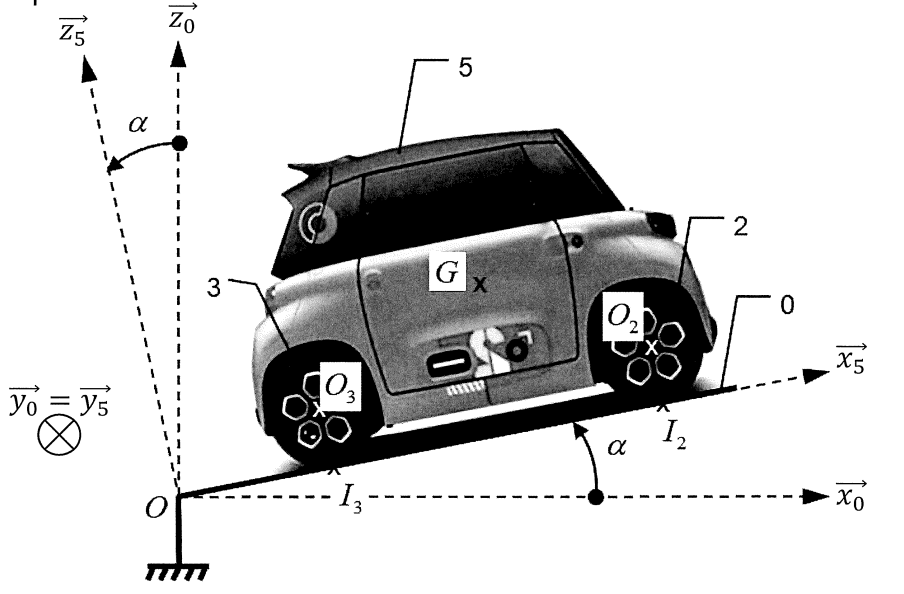
\includegraphics[width=0.75\linewidth]{img/fig19.png}
\caption{\label{fig19}Modèle pour l'étude dynamique de l'AMI}
\end{figure}

Données :
\begin{itemize}
  \item le châssis 5 est de masse $m_5$, de centre de gravité $G$ ;
%  \item l'essieu avant 2 est de masse $m_2$, de centre de gravité $O_2$ et de moment d'inertie $J_2$ autour de l'axe $(O_2,\overrightarrow{y_0})$ ;
  \item l'essieu avant 2 est de masse $m_2$, de centre de gravité $O_2$ et son moment d'inertie est négligé ;
  \item l'essieu arrière 3 est de masse $m_3$, de centre de gravité $O_3$ et son moment d'inertie est négligé.
\end{itemize}

Hypothèses :
\begin{itemize}
  \item $\overrightarrow{z_0}$ est vertical ascendant ;
  \item le repère lié au sol $(O,\overrightarrow{x_0},\overrightarrow{y_0},\overrightarrow{z_0})$ est galiléen ;
  \item les roues roulent sans glisser sur le sol en $I_2$ et $I_3$ ;
  \item le déplacement du véhicule est suivant $+\overrightarrow{x_5}$ ;
  \item toutes les liaisons sont parfaites à l'exception du contact entre les roues avant et le sol et la liaison pivot entre l'essieu avant et le châssis.
\end{itemize}

Le mouvement du véhicule par rapport au sol est imposé par le torseur cinématique suivant :$\{V_{5/0}\} = \left\{\begin{array}{c} V\cdot\overrightarrow{x_5} \\ \overrightarrow{0} \end{array}\right\}_{G}$. On note $\omega_{25}$ la vitesse angulaire des roues avant par rapport au châssis et $\omega_{35}$ la vitesse angulaire des roues arrière par rapport au châssis. Avec dans notre cas, $\omega_{25} = \omega_{35} = \omega$.

\textbf{Liaison pivot essieu avant / châssis :} La liaison pivot entre l'essieu avant et le châssis est considérée non parfaite. L'action de frottement dans cette liaison est modélisé par un couple constant sur l'axe :$\{T_{f\to 2}\} = \left\{\begin{array}{c} \overrightarrow{0} \\ C_f\cdot\overrightarrow{y_0} \end{array}\right\}_{O_2} \quad \text{avec } C_f < 0.
$

\textbf{Contact sol / roues avant :} Les contacts au sol des roues avant sont modélisés avec du frottement sec de modèle de Coulomb. Ainsi l'effort de contact entre le sol 0 et l'essieu avant 2 est modélisé par le torseur suivant :$\{T_{0\to 2}\} = \left\{\begin{array}{c} T_2\cdot\overrightarrow{x_5} + N_2\cdot\overrightarrow{z_5} \\ \overrightarrow{0} \end{array}\right\}_{I_2}$. Le facteur de frottement entre le sol et les roues est noté $\mu$ avec $\mu = 0.9$.

\textbf{Couple moteur sur les roues avant :} L'énergie mécanique de rotation développée par le moteur est transmise à l'essieu avant via la transmission et le différentiel. Le couple moteur exercé par le différentiel sur l'essieu avant est noté $C_{roue}$. L'effort moteur sur l'essieu avant 2 est donc modélisé par le torseur couple suivant :$\{T_{m\to 2}\} = \left\{\begin{array}{c} \overrightarrow{0} \\ C_{roue}\cdot\overrightarrow{y_0} \end{array}\right\}_{O_2}$.

\textbf{Effets aérodynamiques :} Les effets aérodynamiques exercent une résistance à l'avancement proportionnelle au carré de la vitesse du véhicule par rapport au sol. Ainsi, cet effort sera modélisé par le torseur suivant :
$\{T_{aero\to(5,2,3)}\} = \left\{\begin{array}{c} -K\cdot V^2\cdot\overrightarrow{x_5} \\ \overrightarrow{0} \end{array}\right\}_{C}$. Le centre de poussée $C$ est tel que $\overrightarrow{GC} = c\cdot\overrightarrow{z_5}$. Le coefficient $K$ sera considéré constant pendant l'étude.

\medskip
Le théorème de la résultante dynamique appliqué au véhicule et projeté sur l'axe $\vec{x_5}$ donne :

\begin{center}
$M\cdot\dfrac{dV}{dt}=\sum \vec{F}\cdot \vec{x_5}$, avec $M$ la masse totale de la voiture.
\end{center}

\medskip
Le théorème du moment dynamique appliqué à l'essieu avant et projeté sur l'axe $\vec{y_5}$ donne :

\begin{center}
$\sum \vec{C}\cdot \vec{y_5}=0$, l'inertie $J_2$ de l'essieu étant négligée.
\end{center}

L'ensemble des valeurs numériques nécessaires sont portées dans le tableau \ref{tab02} :

\begin{table}[!ht]
\begin{center}
\begin{tabular}{|c|c|c|}
\hline
$K = 0.2N\cdot m^{-1}\cdot s^2$ & $\alpha = -3\degree$ ($\sin 3\degree\approx 0.05$) & $R = 0.275m$ \\
\hline
$C_f = -3N\cdot m$ & $\mu = 0.9$ & $M = m_5 + m_2 + m_3 = 640kg$ \\
\hline
\end{tabular}
\caption{\label{tab02}Données numériques}
\end{center}
\end{table}

\begin{figure}[!ht]
\begin{center}
 \def\svgwidth{.5\linewidth}
 \input{img/fig12.pdf_tex}
\end{center}
\caption{\label{fig12}Transmission entre le moteur et la roue}
\end{figure}

\medskip
Lors d'un essai sur route, on mesure une vitesse de rotation du moteur de $6694tr\cdot min^{-1}$ pour une vitesse du véhicule de $45km\cdot h^{-1}$.

\question{Justifier ce résultat à l'aide des données du tableau \ref{tab02} et de la figure \ref{fig12} et déterminer la valeur numérique du rapport de la transmission $r = \dfrac{V}{\omega_{moteur}}$.}

\question{En justifiant de l'isolement utilisé, et en effectuant une démonstration complète, montrer que $R\cdot T_2=C_{roue}+C_f$.}

\question{Effectuer le bilan des actions mécaniques extérieures au système isolé $\Sigma = (5,2,3)$.}

\question{En appliquant le principe fondamental de la dynamique à l'ensemble $\Sigma = (5,2,3)$ projeté sur l'axe $\vec{x_5}$, déterminer l'expression du couple sur les roues $C_{roue}$ et le mettre sous la forme $C_{roue} = A\cdot\dfrac{dV}{dt} + B\cdot V^2 + C$. Déterminer les trois constantes $A$, $B$ et $C$ en fonction des constantes du problème.}

\medskip Le modèle dynamique ainsi obtenu, nous cherchons à vérifier la valeur maximale du couple moteur à fournir dans la phase d'accélération. Nous opterons pour une loi de vitesse trapézoïdale théorique suivante (figure \ref{fig20}).

\begin{figure}[H]
\centering
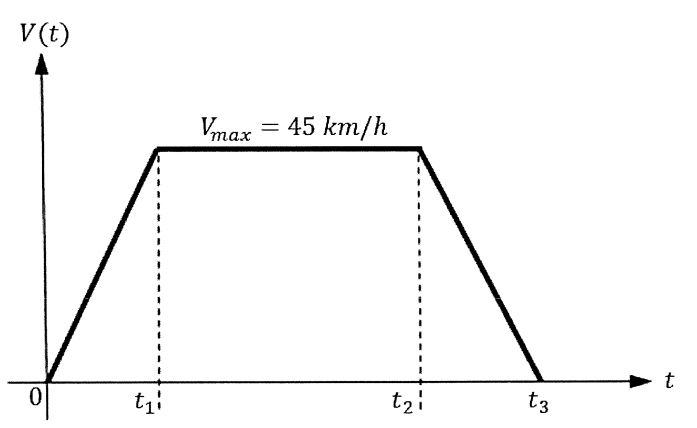
\includegraphics[width=0.5\linewidth]{img/fig20.png}
\caption{\label{fig20}Loi de vitesse trapézoïdale}
\end{figure}

Le constructeur indique que le $0\rightarrow 45km\cdot h^{-1}$ est réalisé en 10s.

\question{Déterminer la valeur de l'accélération du véhicule $\gamma = \dfrac{dV}{dt}$ dans la première phase du mouvement.}

\question{En justifiant l'instant choisi, déterminer la valeur maximale du couple sur les roues $C_{roue}$ à fournir pour suivre la loi de vitesse. Faire l'application numérique.}

\medskip
On suppose que le rendement de la transmission est unitaire et le couple maximum du moteur est de $65N\cdot m$.

\question{Conclure sur la capacité du moteur à respecter le $0\rightarrow 45km\cdot h^{-1}$ en 10s et donc à respecter l'exigence 1.3.3.}

\section{Contrôle du couple moteur pour valider l'exigence 1.3.3}

\textbf{Objectif :} \textit{valider les performances de la boucle de courant pour contrôler la vitesse et le couple du moteur.}

\medskip
C'est le contrôle du couple instantané $C_{em}$ du moteur qui permet de contrôler la vitesse et le couple, y compris en régime transitoire. Ce contrôle est délicat puisqu'il dépend des courants instantanés des 3 phases et de la position du rotor obtenue par le traitement des signaux issus du capteur angulaire.

\noindent On préfère alors utiliser une commande plus rapide et plus efficace qui se ramène à l'étude d'un cas diphasé fictif équivalent grâce à un modèle mathématique adapté (transformation de Park) dans le plan « dq » (d pour direct et q pour quadrature).

\medskip
Afin de minimiser les pertes Joule avec un courant $I$ minimum correspondant à un angle $\psi = 0$, on choisit alors d'asservir le courant $i_d(t)$ à une valeur nulle.

\medskip
On obtient alors les équations suivantes en négligeant les frottements :
\begin{align}
V_q(t) &= R_{eq}\cdot i_q(t) + L_{eq}\cdot\frac{di_q(t)}{dt} + K_E\cdot\omega_m(t) \tag{équation 1}\\
C_{em}(t) &= K_T\cdot i_q(t) = J_{eq}\frac{d\omega_m(t)}{dt} \tag{équation 2}
\end{align}

\medskip
\noindent Avec :
\begin{itemize}
  \item $L_{eq}$ (H) : Inductance équivalente d'induit sur l'axe d supposée égale à celle sur l'axe q
  \item $R_{eq}$ ($\Omega$) : Résistance équivalente d'enroulement statorique
  \item $J_{eq}$ (kg.m²) : Inertie équivalente ramenée au rotor moteur
  \item $\omega_m$ (rad.s$^{-1}$) : vitesse de rotation du rotor
  \item $C_{em}(t)$ (N.m) : couple électromagnétique supposé égal au couple moteur
  \item $K_E$ (V.s.rad$^{-1}$) : constante de fem
  \item $K_T$ (N.m/A) : constante de couple
  \item $V_q(t)$ (V) : tension d'alimentation de la phase fictive en quadrature
\end{itemize}

\medskip
Le schéma de principe de l'asservissement de courant devient celui donné sur la figure \ref{fig23}.

\begin{figure}[!ht]
\centering
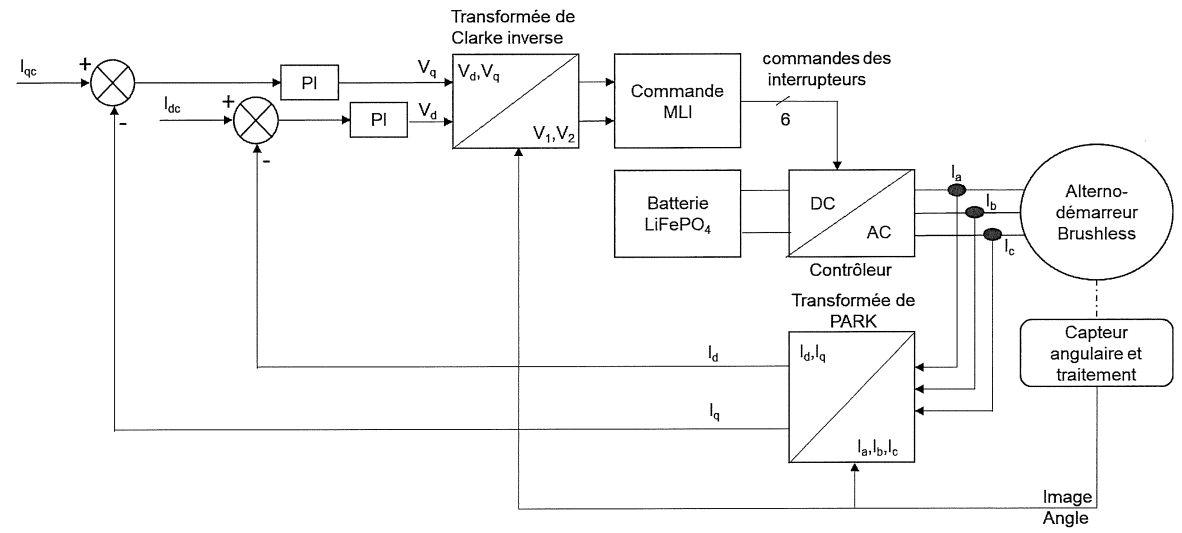
\includegraphics[width=0.7\linewidth]{img/fig23.png}
\caption{\label{fig23}Principe de l'asservissement en courant}
\end{figure}

\medskip
Nous supposerons pour la suite que $I_d$ est parfaitement asservi à la valeur $I_{dc} = 0$ et nous nous intéresserons à l'asservissement du courant $I_q$.

\begin{center}
\begin{tabular}{|m{0.1\linewidth}|m{0.65\linewidth}|m{0.18\linewidth}|}
\hline
\textbf{Exigence} & \textbf{Critère} & \textbf{Performance attendue} \\
\hline
Précision & Erreur relative en régime permanent vis-à-vis d'un échelon de consigne de valeur $I_{qc0}$ & $\varepsilon_\infty \leq 2\%$ \\
\hline
\end{tabular}
\end{center}

\medskip
Dans ces conditions, nous pouvons formaliser les boucles d'asservissement au moyen de techniques développées pour les systèmes linéaires.

\question{Exprimer $V_q(p)$ ainsi que $C_{em}(p)$ dans le domaine de Laplace à partir des équations temporelles fournies (équation 1) et (équation 2) et en déduire les expressions de $H_1(p)$ et $H_2(p)$ dans le schéma bloc de la figure  \ref{fig24}.}

\newpage

\begin{figure}[!ht]
\centering
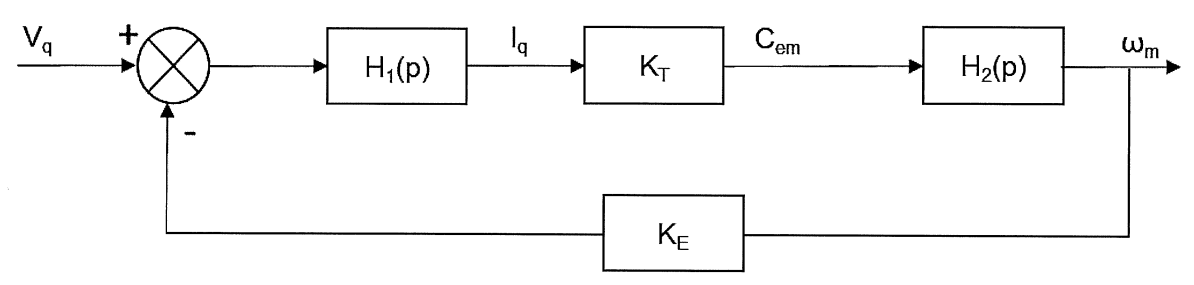
\includegraphics[width=0.7\linewidth]{img/fig24.png}
\caption{\label{fig24}Schéma bloc}
\end{figure}

\question{En déduire la fonction de transfert $T(p) = \dfrac{I_q(p)}{V_q(p)}$ sous forme canonique.}

\medskip
Pour la suite des questions, on prendra :$T(p) = \frac{T_0\cdot p}{\left(1 + \dfrac{2m}{\omega_0}\cdot p + \dfrac{p^2}{\omega_0^2}\right)}$ avec $T_0 = 2\,\Omega^{-1}$\text{.s}.


\medskip
La boucle d'asservissement de courant se ramène à l'étude du schéma bloc de la figure \ref{fig25} :

\begin{figure}[!ht]
\centering
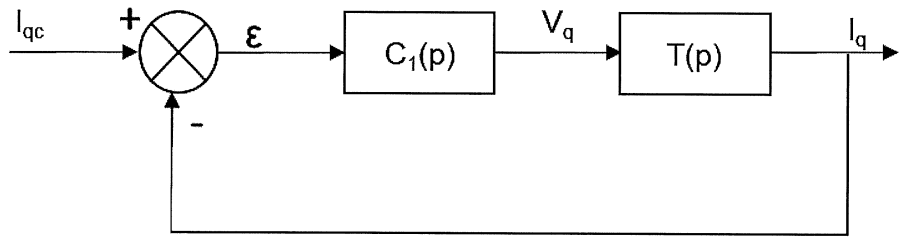
\includegraphics[width=0.5\linewidth]{img/fig25.png}
\caption{\label{fig25}Schéma bloc de l'asservissement en courant}
\end{figure}

\medskip
$C_1(p)$ représente le correcteur PI de fonction de transfert :
\[
C_1(p) = K_1\cdot\frac{1 + \tau_i\cdot p}{\tau_i\cdot p}
\]
\question{Déterminer l'erreur relative en régime permanent $\varepsilon_\infty$ pour une consigne en échelon de courant d'amplitude $I_{qc0}$ puis déterminer la valeur de $K_1$ à choisir vis-à-vis des exigences de l'asservissement de courant en terme de précision en choisissant une valeur de $\tau_i = T_0$.}

\section{Étude de la fabrication du support d’axe mobile}

Cette partie a pour objectif de vérifier la faisabilité du support d’axe mobile, dont le dessin de définition, est donné sur le document ressource DT5. Cette pièce intervient dans la réalisation des liaisons pivots et sert également de support au système de suspension. Pour la fabrication du prototype, le brut de la pièce a été obtenu par moulage.

\question{Quelles doivent être les propriétés physiques de la pièce « support d’axe mobile », permettant d’assurer un fonctionnement correct du mécanisme ?}

\question{Dans le cadre d’une fabrication en grande série, quel procédé d’obtention de brut serait plus en rapport avec les caractéristiques demandées à la question précédente ? Expliquer succinctement ce procédé et énoncer les règles de tracé.}

\question{À partir des informations du dessin de définition partiel du document ressource DT5, interpréter la spécification suivante : $336\pm0.3$.}

\question{À partir des informations du document DT5, interpréter la spécification suivante. \begin{center}
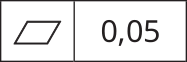
\includegraphics[height=0.03\textheight]{img/fig26}
\end{center}}

\question{À partir des informations du document DT5, interpréter la spécification suivante. \begin{center}
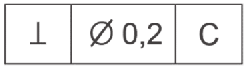
\includegraphics[height=0.03\textheight]{img/fig27}
\end{center}}

\question{À partir des informations du document DT5, interpréter la spécification suivante. \begin{center}
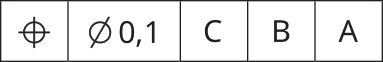
\includegraphics[height=0.03\textheight]{img/fig28}
\end{center}}

%%%%%%%%%%%%%%%%%%%%%%%%%%%%%%%%%%%%%%%%%%%%%%%%%%%%%%%%%%%%%%%%%%%%%%%%%%%%%
% DOCUMENTS TECHNIQUES
%%%%%%%%%%%%%%%%%%%%%%%%%%%%%%%%%%%%%%%%%%%%%%%%%%%%%%%%%%%%%%%%%%%%%%%%%%%%%
\newpage
\begin{center}
  {\large\bfseries Document technique DT1 : Fonctionnement général de la voiture}
\end{center}

\begin{center}
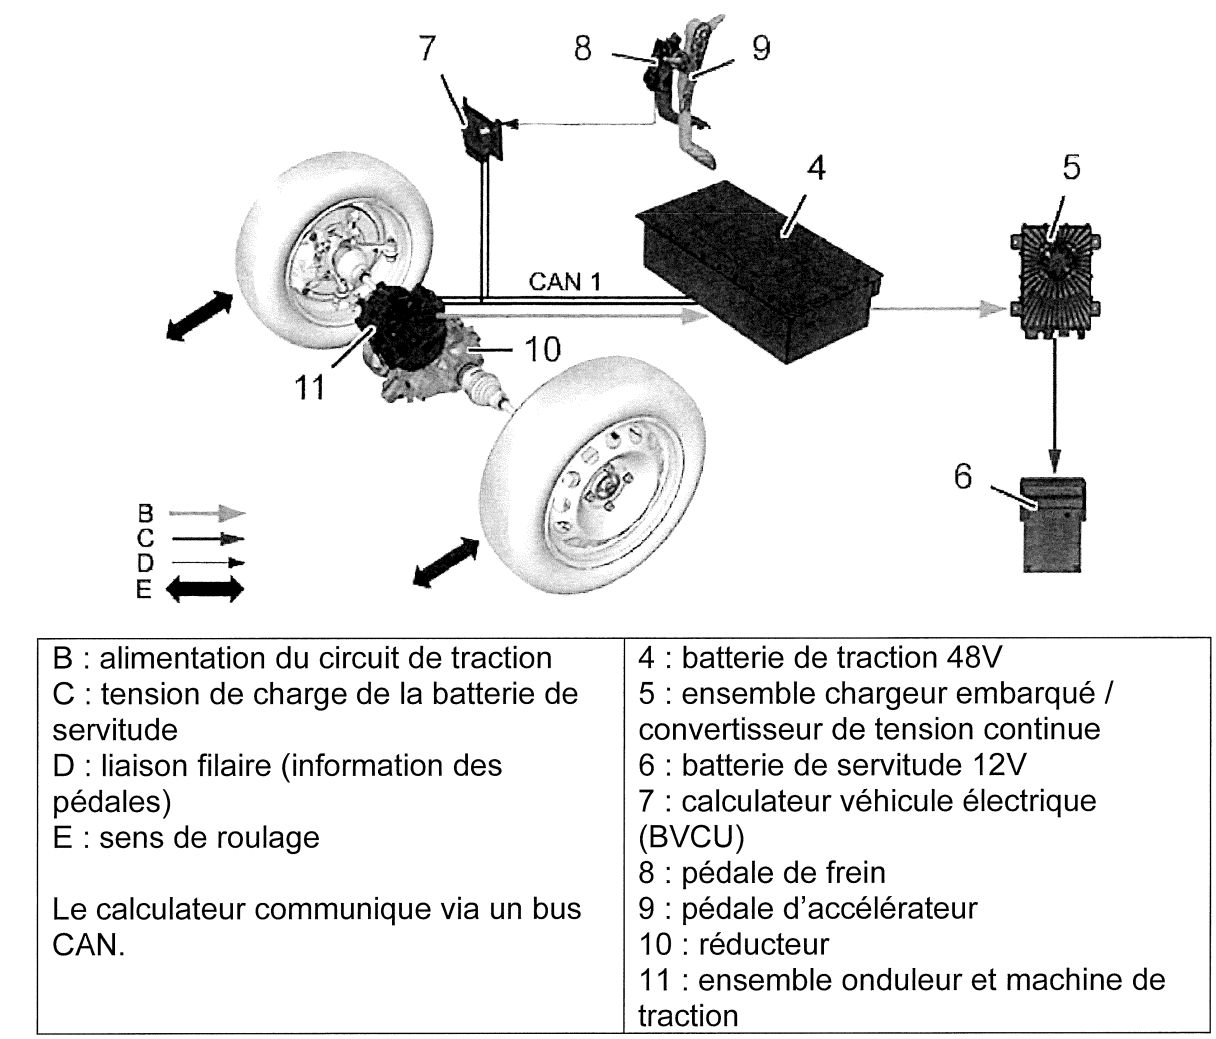
\includegraphics[width=0.8\linewidth]{img/DT01.png}

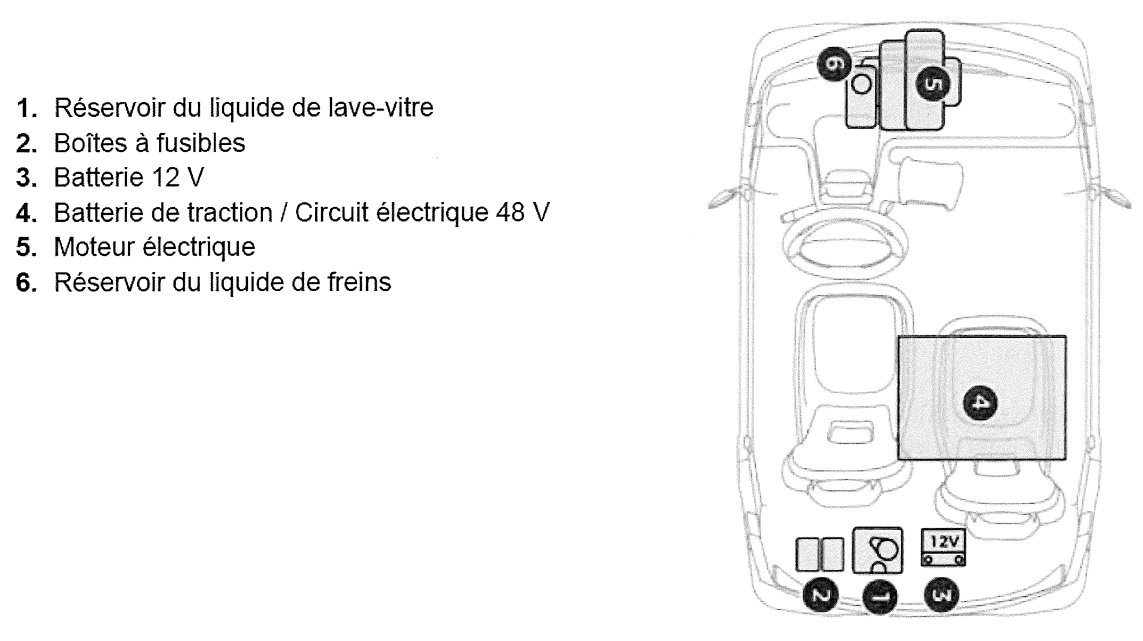
\includegraphics[width=0.8\linewidth]{img/DT02.png}
\end{center}

\newpage

\begin{center}
  {\large\bfseries Document technique DT2 : Bus CAN}
\end{center}

\begin{minipage}{0.55\linewidth}
Le bus CAN est utilisé dans de nombreux domaines, automobile, agricole, industriel, médical\ldots{} Ce bus de terrain est économique et évolutif, sa vitesse de transmission peut atteindre 1 Mbit/s. Dans notre étude elle est de 500 kbit/s.

\medskip
Chaque équipement connecté, ou « nœud », peut communiquer avec tous les autres.\end{minipage}
\hfill
\begin{minipage}{0.42\linewidth}
  \centering
  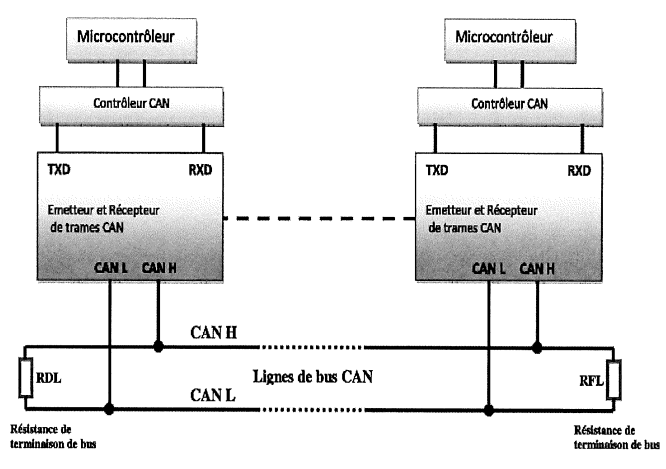
\includegraphics[width=0.9\linewidth]{img/DT03.png}
\end{minipage}

\medskip
L'accès au bus CAN suit la technique \textbf{CSMA/CD} (écoute de chaque station avant de parler mais pas de tour de parole, résolution des collisions par priorité).

\medskip
En cas d'émission simultanée de plusieurs stations, l'attribution du bus suit le principe d'arbitrage suivant en comparant bit à bit l'identificateur de leur message (ID) avec celui des messages concurrents.

Pour cela les stations sont câblées sur le bus par le principe du ``ET câblé''.

En cas de conflit, c'est à dire d'émissions simultanées, la valeur 0 d'un émetteur impose le potentiel de bus à « 0 » l'état 1 est « écrasé »\ldots

On appelle donc \textbf{``état dominant''} l'état logique 0, et \textbf{``état récessif''} l'état logique 1.

\begin{minipage}{0.55\linewidth}
Lors de l'arbitrage bit à bit, dès qu'une station émettrice se trouve en état récessif et détecte un état dominant, « elle perd » et arrête d'émettre.

Les ID de priorités moins élevée perdent la compétition face à celle qui a la priorité la plus élevée. Tous les perdants deviennent automatiquement des récepteurs du message, et ne tentent à nouveau d'émettre que lorsque le bus se libère. Pour un véhicule par exemple, tout ce qui est lié à la sécurité est de haute priorité par rapport à la climatisation, \ldots
\end{minipage}
\hfill
\begin{minipage}{0.42\linewidth}
  \centering
  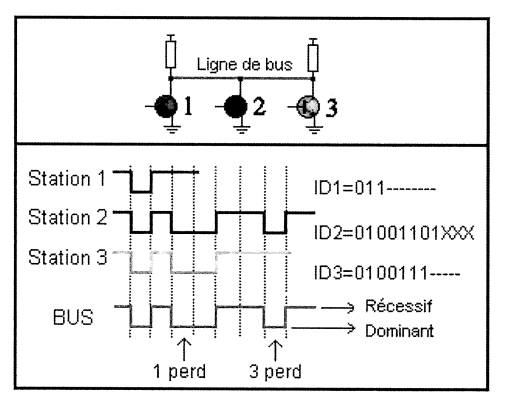
\includegraphics[width=0.9\linewidth]{img/DT04.png}
\end{minipage}

\medskip
\noindent\textbf{Structure Générale d'une trame CAN}

\begin{center}
\begin{tabular}{|p{1cm}|p{2cm}|p{3cm}|p{2.5cm}|p{2cm}|p{1cm}|p{2.5cm}|}
\hline
SOF & Champ d'arbitrage & Champ de commande & Champ de données & Champ de CRC & ACK & EOF \& IFS \\
\hline
1 bit & 12 bits & 6 bits & de 0 à 64 bits & 16 bits & 2 bits & 7 bits \& 3 bits \\
\hline
\end{tabular}
\end{center}

\medskip
Les champs sont transmis dans l'ordre du SOF à l'EOF. Dans chaque champ de la trame, les bits sont transmis du plus fort au plus faible.

\noindent Une trame de données se compose de 7 champs différents :
\begin{itemize}
  \item Le début de trame ou SOF (Start Of Frame) matérialisé par 1 bit dominant (remporte en cas de conflit 0/1),
  \item Le champ d'arbitrage (identificateur des constituants sur 11 bits) + 1 bit RTR fixe le niveau de priorité du message,
  \item Le champ de commande (ou de contrôle) composé de 2 bits qui indique l'action (lecture, écriture\ldots) et 4 bits indiquant le nombre d'octets de données,
  \item Le champ de données composé de 0 à 64 bits (de 0 à 8 octets),
  \item Le champ de CRC composé de 16 bits (contrôle d'erreur) calculé sur les 19 à 101 bits précédents,
  \item Le champ d'acquittement ACK composé de 2 bits,
  \item La fin de trame ou EOF (End of Frame) matérialisée par 7 bits récessifs.
  \item Pour éviter les perturbations, on ajoute en fin de trame un espace inter frame (IFS) de 3 bits récessifs.
\end{itemize}

\medskip
Pour un bus « \textbf{CAN HIGH SPEED} » les niveaux sont définis par rapport à 2,5V et sont donnés ci-contre.

\medskip
En lisant (CANH-CANL) on a donc une image du bit (1 pour 0V et 0 pour 2V).

\begin{center}
\begin{tabular}{|c|c|c|c|}
\hline
\textbf{Niveau} & \textbf{CANH / masse} & \textbf{CANL / masse} & \textbf{CANH - CANL} \\
\hline
Récessif ou « 1 » & 2,5 V & 2,5 V & 0 V \\
\hline
Dominant ou « 0 » & 3,5 V & 1,5 V & 2 V \\
\hline
\end{tabular}
\end{center}

\begin{center}
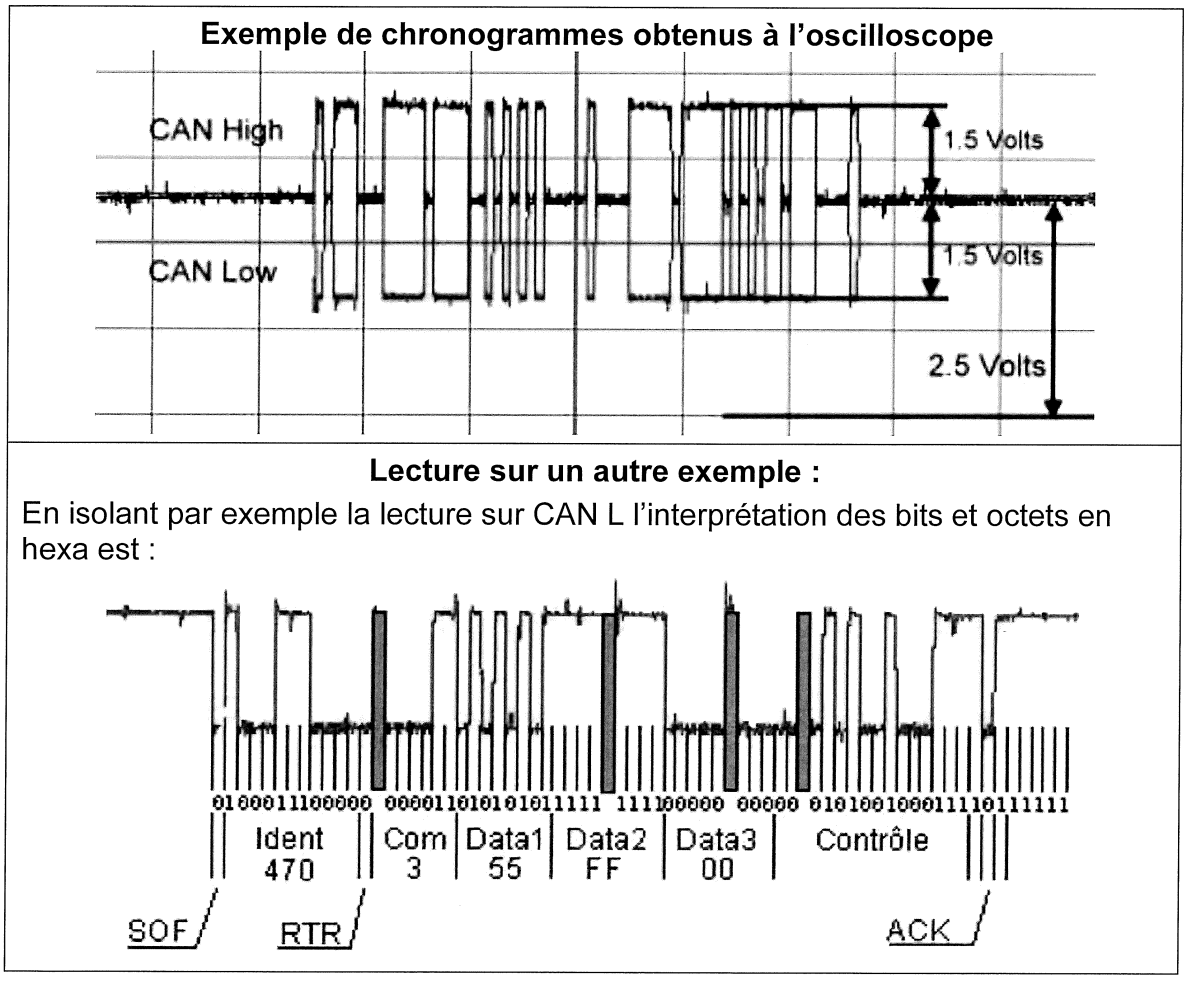
\includegraphics[width=0.7\linewidth]{img/DT07.png}
\end{center}

\medskip
On doit aussi ajouter des bits de stuffing pour éviter des erreurs de transmission, mais pour simplifier, ils ne sont pas à prendre en compte dans les trames du sujet.

\newpage

\begin{center}
  {\large\bfseries Document technique DT3 : Pseudo-code de la résolution par dichotomie}
\end{center}

\begin{lstlisting}
//definitions des donnees (mm)
e <- 200
a <- 80
d <- 1235
l <- 465

//definitions des variables
alpha : flottant
y     : flottant
eps   : flottant

//definition de la fonction a annuler
f <- (e - a*sin(alpha))^2 + (a*cos(alpha) - d/2 + y)^2 - l^2

//algorithme de dichotomie
eps <- 1
Tant que eps > 0.001
    m   <- (u + v) / 2
    eps <- |v - u|
    Si (f(u,y)*f(m,y) <= 0) alors
        v <- m
    sinon
        u <- m
    Fin Si
Fin Tant que
\end{lstlisting}

\begin{center}
  {\large\bfseries Document technique DT4 : Fonction tan}
\end{center}

\begin{figure}[!ht]
\begin{center}
  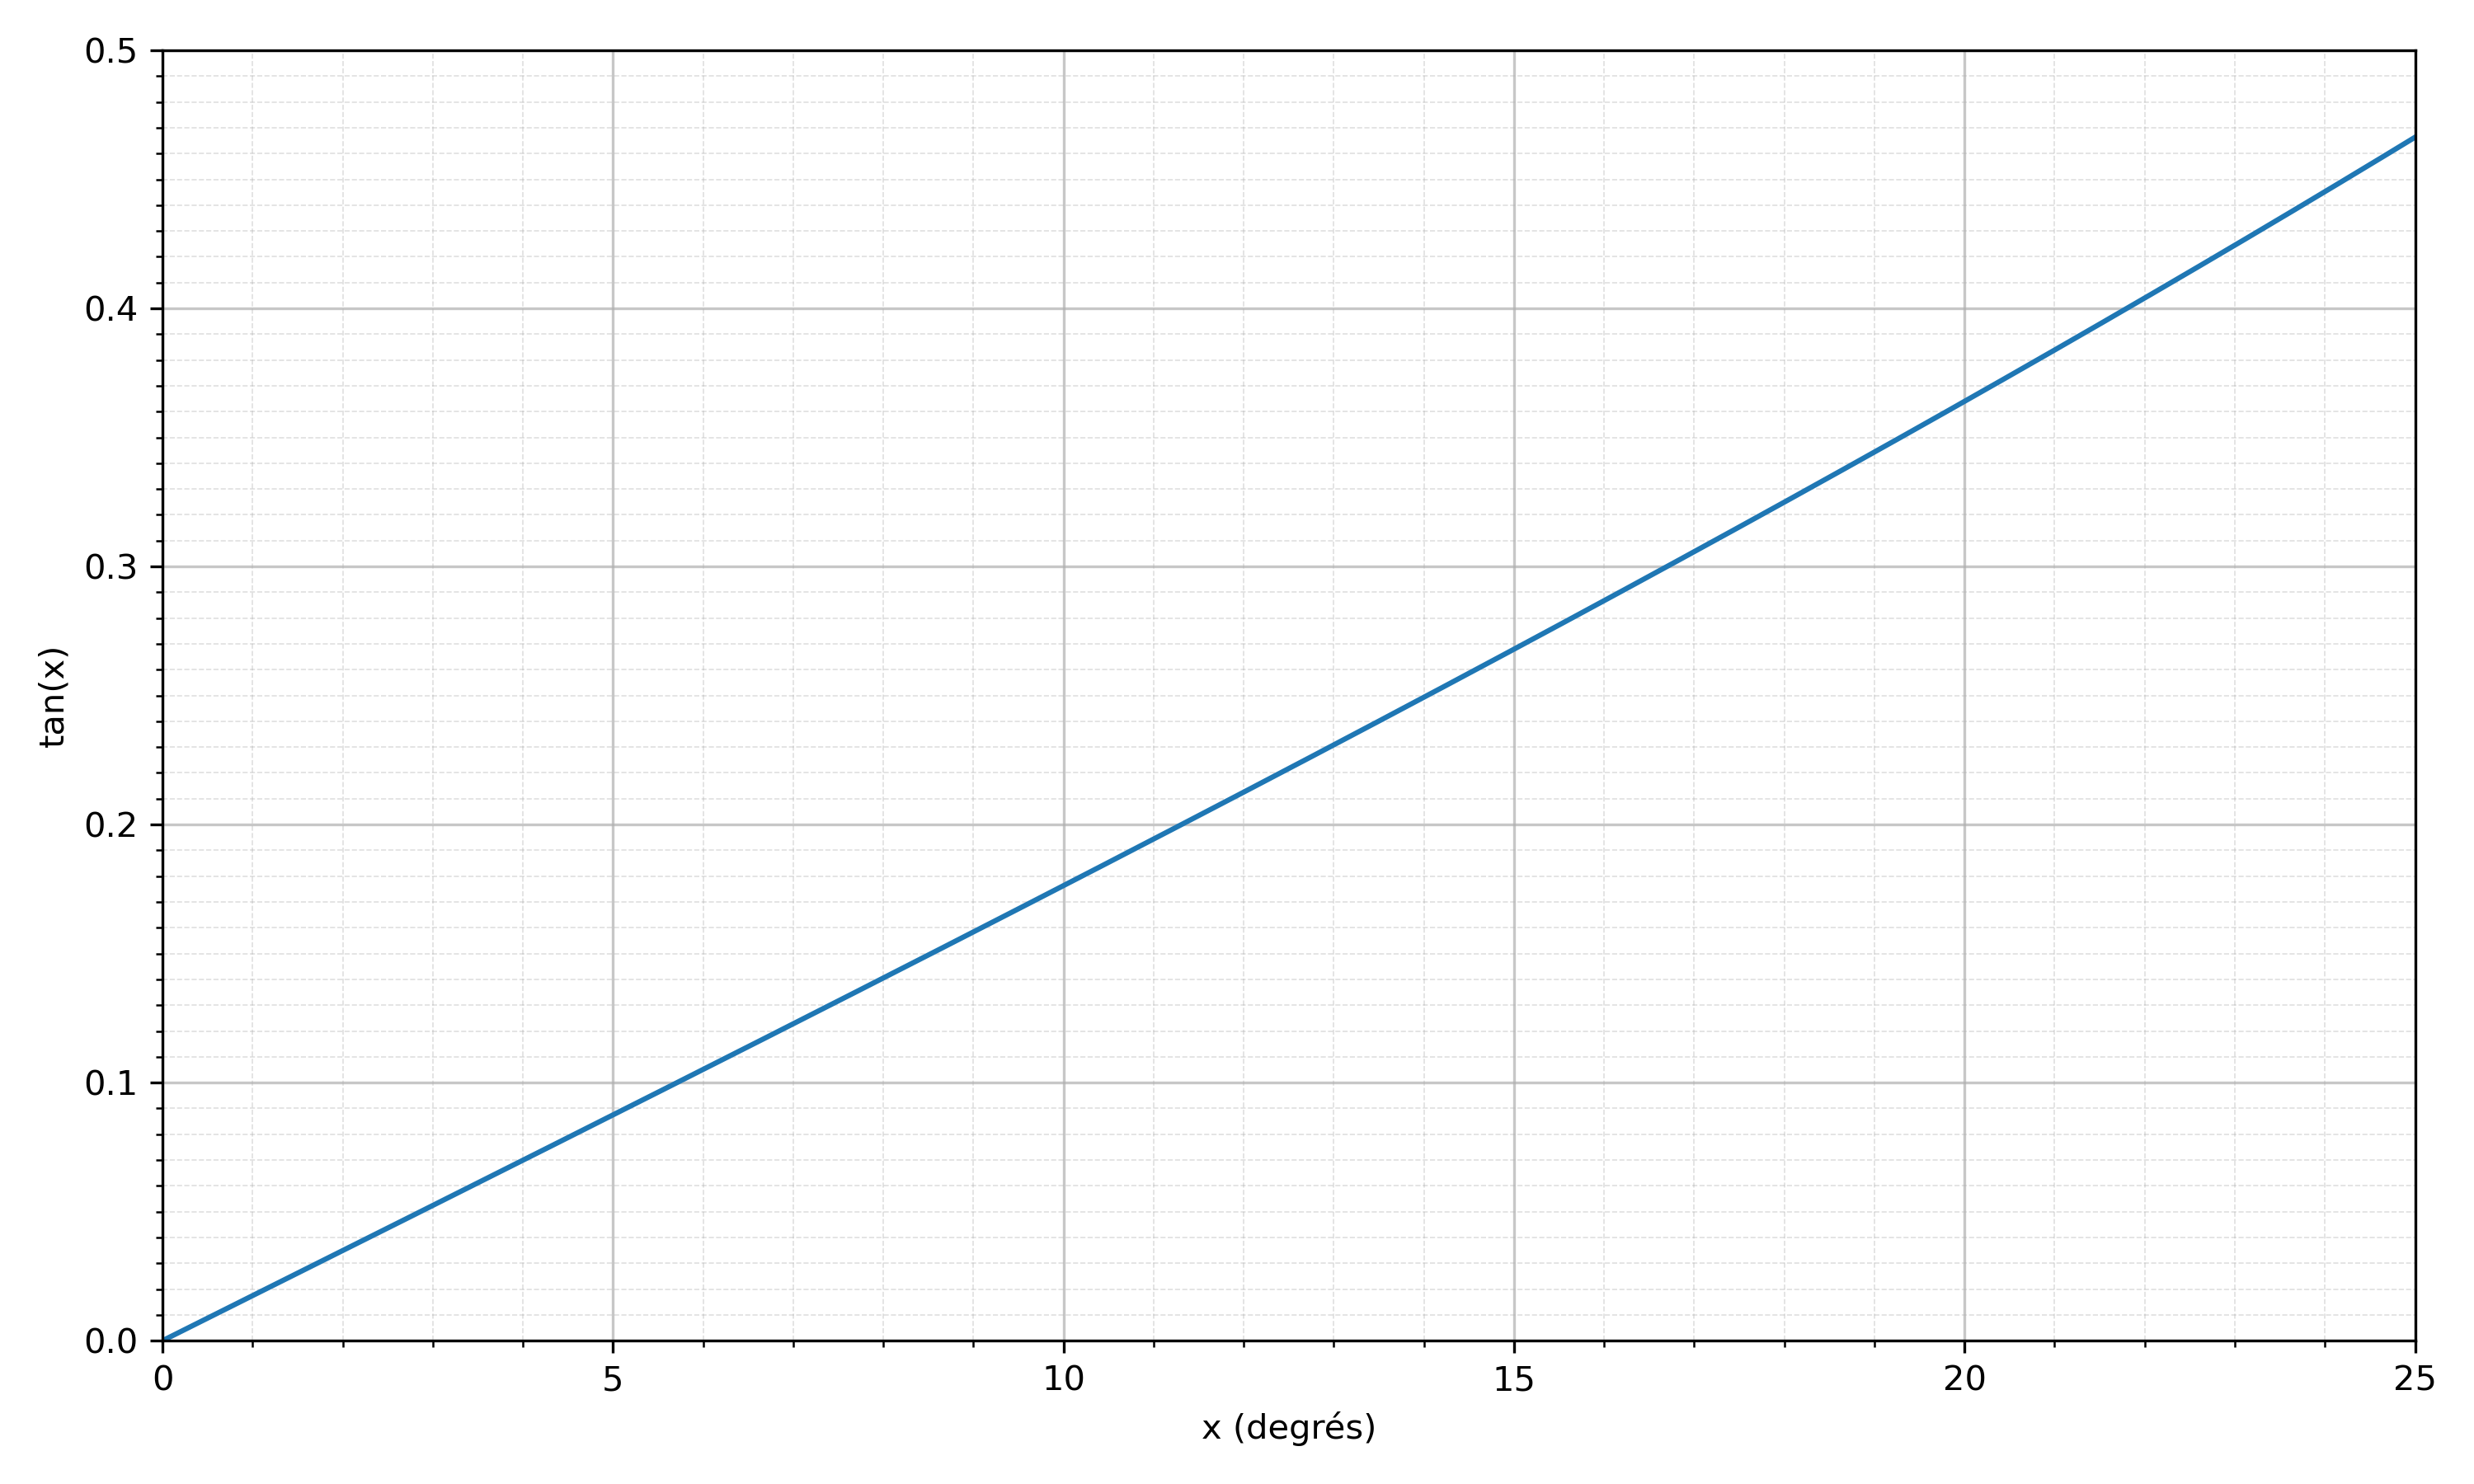
\includegraphics[width=.85\linewidth]{img/DT08.png}
\end{center}
\caption{\label{DT08}Fonction tan(x)}
\end{figure}

\begin{center}
  {\large\bfseries Document technique DT5 : Dessins du support d'axe mobile et de l'ensemble mobile}
\end{center}

\begin{figure}[!ht]
\begin{center}
  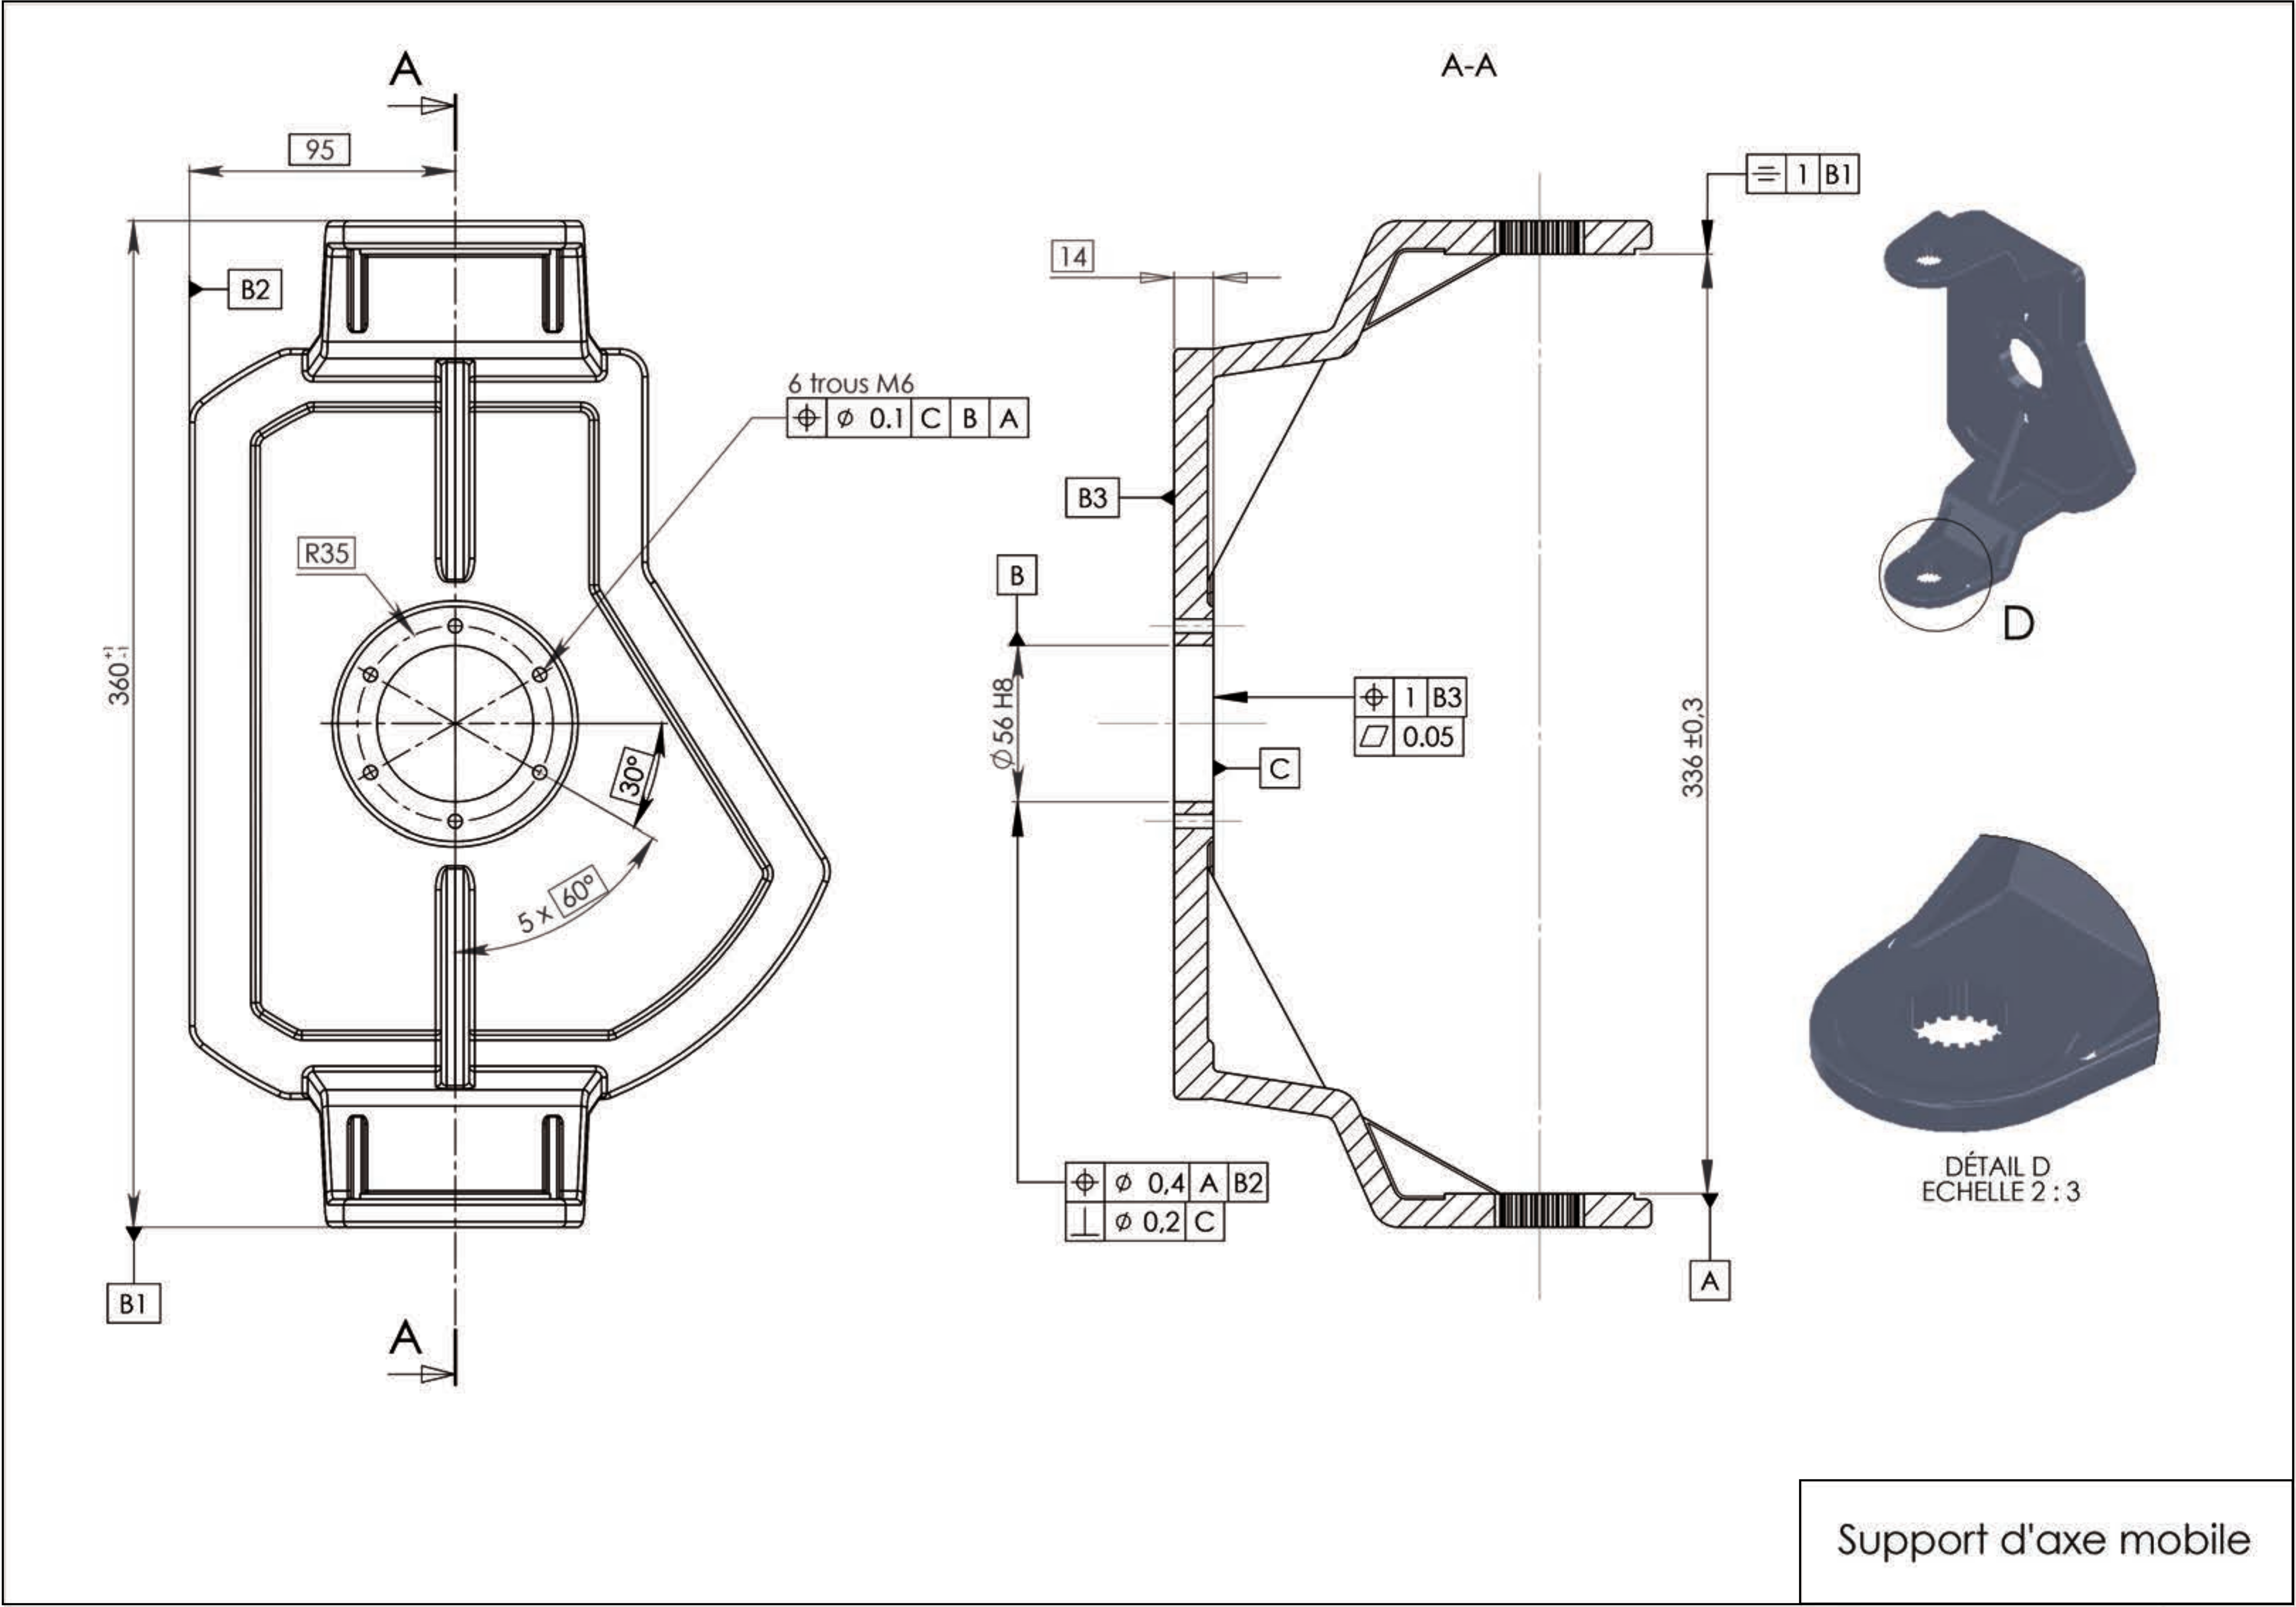
\includegraphics[width=.85\linewidth]{img/DT09.png}\\
  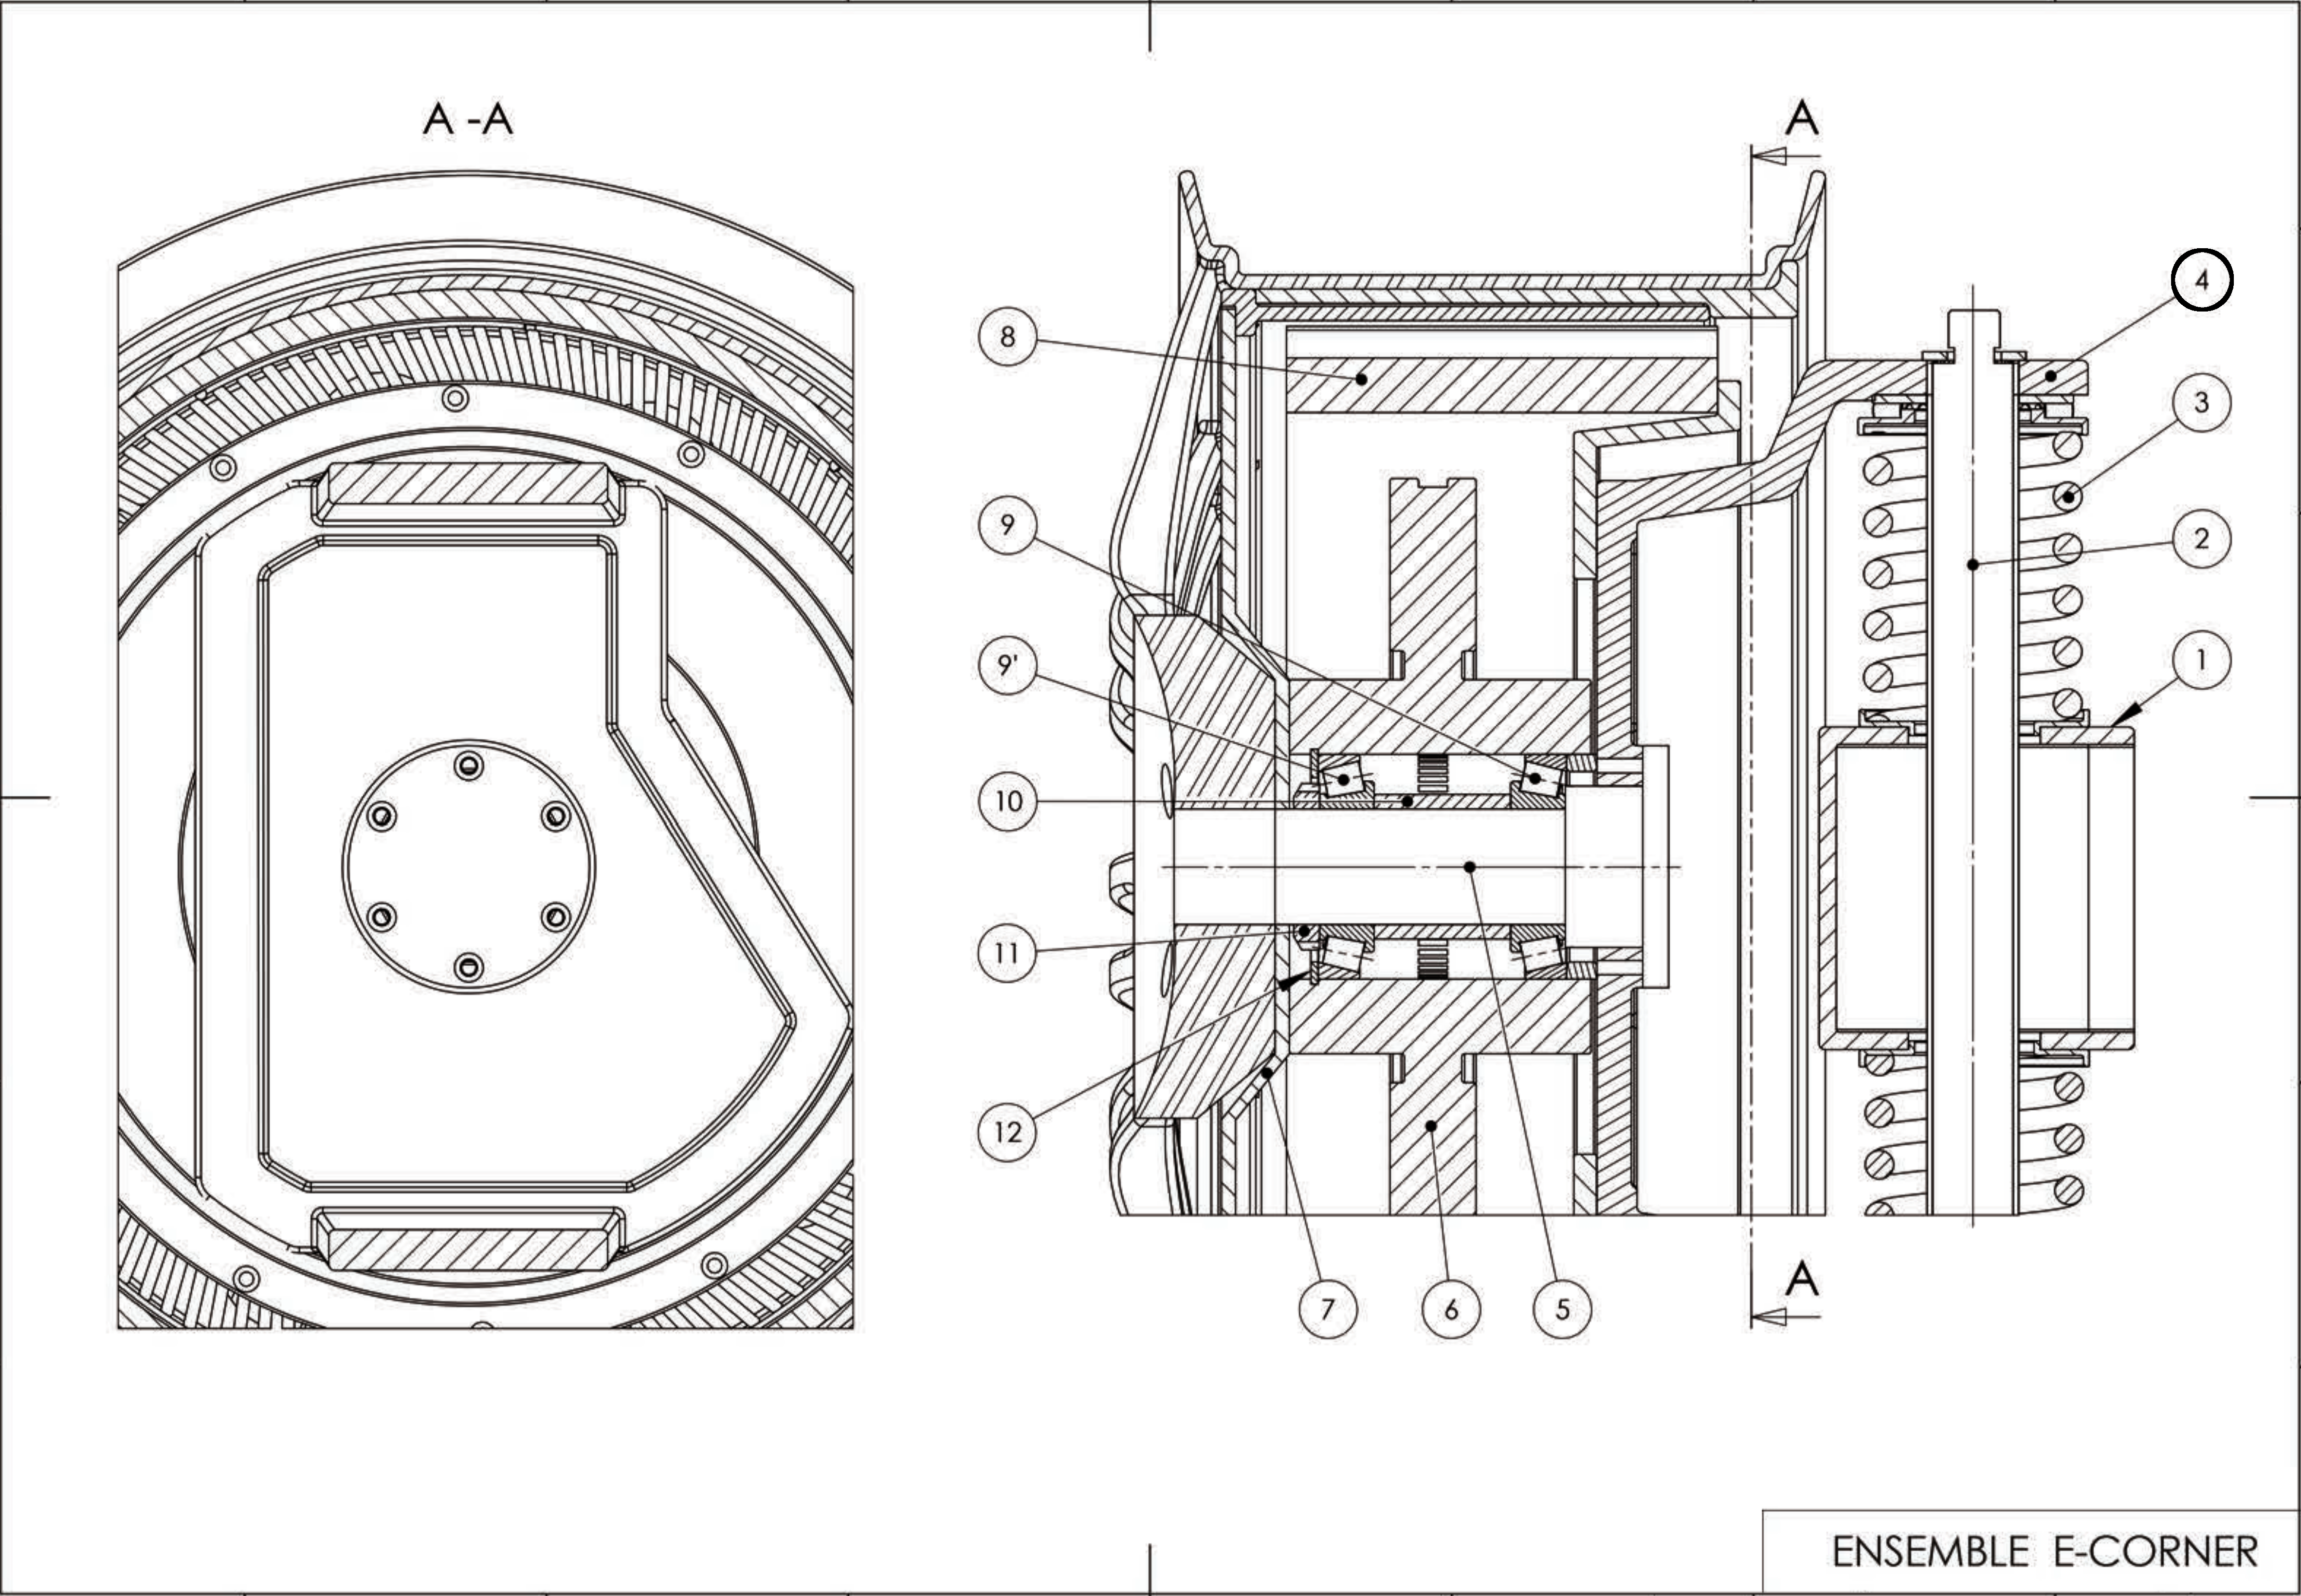
\includegraphics[width=.85\linewidth]{img/DT10.png}
\end{center}
\caption{\label{DT09}Dessins du support d'axe mobile et de l'ensemble mobile}
\end{figure}

\finsujet{public}
%\finsujet

\cleardoublepage

\newpage

\debutcor

\reponse{0}{
\begin{center}
  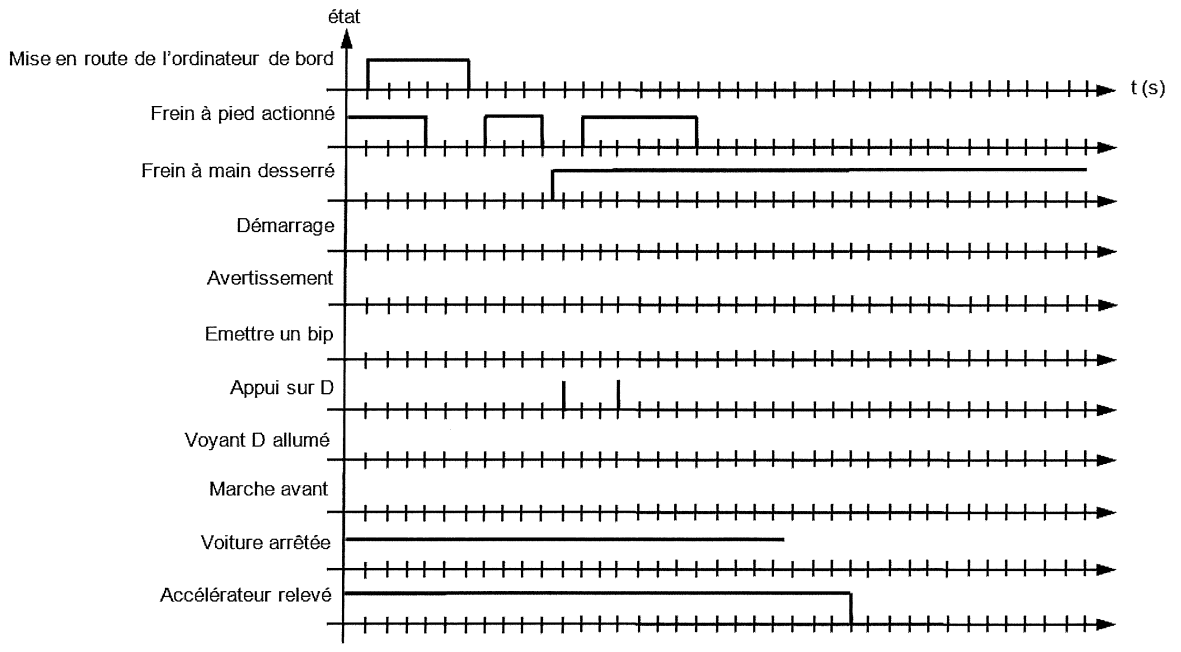
\includegraphics[width=.85\linewidth]{img/DR01.png}
\end{center}
}{
\begin{center}
  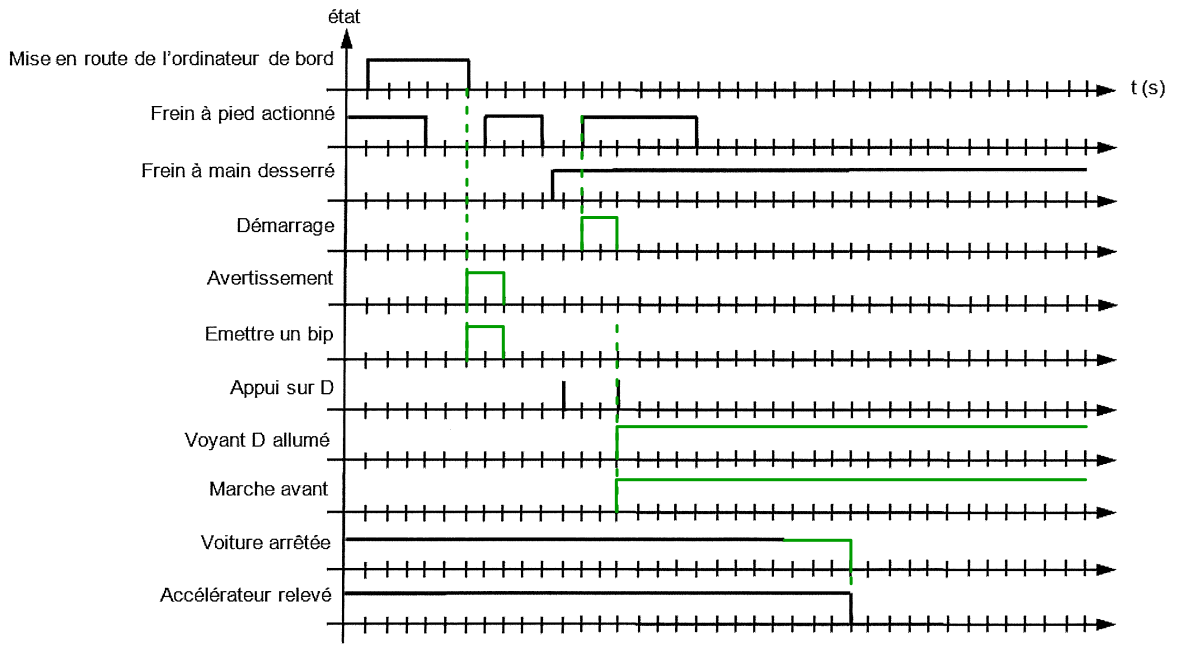
\includegraphics[width=.85\linewidth]{img/DR01_cor.png}
\end{center}
}

\reponse{0}{\begin{center}
  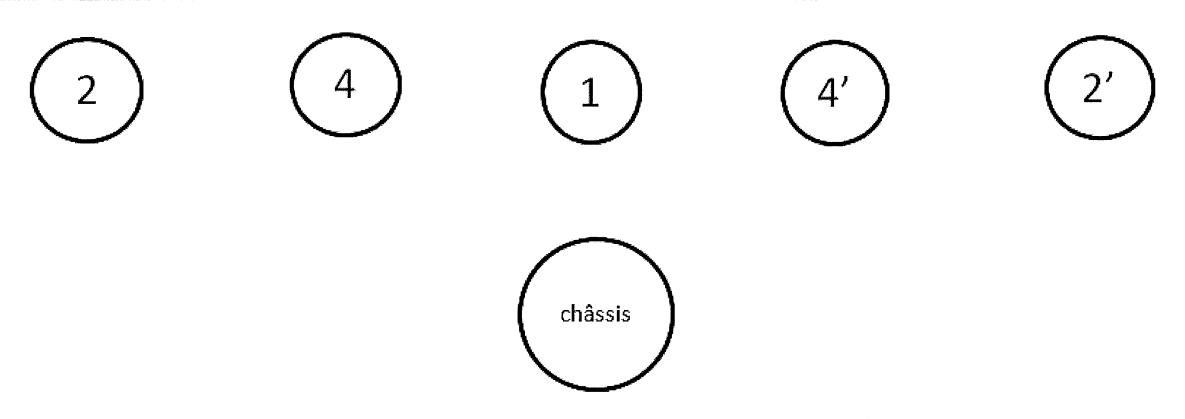
\includegraphics[width=.85\linewidth]{img/DR02.png}
\end{center}}{
\begin{center}
\def\svgwidth{.8\linewidth}
   \input{img/DR02_cor.pdf_tex}
\end{center}
}


\reponse{3}{}{
$h = N_S - 6(p-1) + m$

Avec :
\begin{itemize}
  \item $p = 6$ pièces (châssis, 1, 2, 2', 4, 4')
  \item $N_S = 4\times 5 + 5 + 2\times 3 = 31$
  \item $m=1$
\end{itemize}

$$h = 31 - 30 + 1 = \boxed{2}$$

Le mécanisme est hyperstatique d'ordre 2.
}

\reponse{3}{}{
Pour rendre le mécanisme isostatique ($h = 0$), il faut supprimer 2 degrés d'hyperstatisme.

Remplacer les deux liaisons sphériques (en B ou B') par des linéaires annulaires d'axe ($B,\vec{z_1}$) (respectivement $B',\vec{z_1}$), ou remplacer les liaison pivot (en A ou A') par des liaisons pivot-glissant.}

\reponse{4}{}{
$$\overrightarrow{OB} + \overrightarrow{BA} + \overrightarrow{AO_2} + \overrightarrow{O_2H} + \overrightarrow{HO} = \overrightarrow{0}$$

$$-y(t)\cdot\overrightarrow{y_1} + l\cdot\overrightarrow{x_4} + (-a\cdot\overrightarrow{y_g}) + \frac{d}{2}\cdot\overrightarrow{y_1} + (-e\cdot\overrightarrow{x_1}) = \overrightarrow{0}$$
}

\reponse{4}{}{
$$\overrightarrow{x_4} = \cos\alpha_g\cdot\overrightarrow{x_1} - \sin\alpha_g\cdot\overrightarrow{y_1}$$
$$\overrightarrow{y_g} = -\sin\alpha_g\cdot\overrightarrow{x_1} + \cos\alpha_g\cdot\overrightarrow{y_1}$$

\textbf{Projection sur $\overrightarrow{x_1}$ :}
$$l\cdot\cos\alpha_g + a\cdot\sin\alpha_g - e = 0$$

\textbf{Projection sur $\overrightarrow{y_1}$ :}
$$-y(t) - l\cdot\sin\alpha_g - a\cdot\cos\alpha_g + \frac{d}{2} = 0$$
}


\reponse{3}{}{
D'après la projection sur $\overrightarrow{y_1}$ :
$$\boxed{y(t) = \frac{d}{2} - l\sin\alpha_g(t) - a\cos\alpha_g(t)}$$
}

\reponse{4}{}{
En tournant vers la gauche, on sait que $-90\degree < \alpha_g < 0\degree$.

Ainsi, la solution se trouve entre ces deux valeurs, on peut donc prendre :
\begin{itemize}
  \item $u = -90$
  \item $v = 0$
\end{itemize}
}

\reponse{4}{}{
$\varepsilon = |u - v|$ est le \textbf{critère d'arrêt} (précision) de l'algorithme de dichotomie. 

L'algorithme s'arrête quand $\varepsilon \leq 0.001$ (= 0,001 mm dans notre cas), c'est-à-dire quand l'intervalle $[u, v]$ est suffisamment resserré autour de la solution, garantissant une précision de $10^{-3}$ sur la valeur de $\alpha_g$.}

\reponse{4}{}{
Le volant peut faire 1 tour à partir de la position central avec un rayon pour le pignon de la crémaillère de 15mm.

\begin{itemize}
  \item $y_{min} = 200 - 2\times \pi\ \times 15 \approx 200 - 90 \approx 110$\,mm   \item $y_{max} = 200 + 90 \approx 290$\,mm
\end{itemize}}

\reponse{2}{}{
Les angles de braquage maximal sont donc $|\alpha_{max}| \approx 60°$.
}

\reponse{3}{}{
Par lecture géométrique, on trouve:
\begin{itemize}
 \item $$\tan\alpha_g = \frac{L}{\lambda - d/2}$$
 \item $$\tan\alpha_d = \frac{L}{\lambda + d/2}$$
\end{itemize}
}

\reponse{5}{}{
Avec $L = 1.85$\,m, $d = 1.23$\,m, $\lambda = 7.5$\,m :

$$\tan\alpha_g = \frac{1.85}{7.5 - 0.615}=\frac{1.85}{6.885}\approx 0.2+\frac{0.5}{6.885} \approx 0.27$$

$$\alpha_g = \arctan(0.27) \approx \boxed{15\degree}$$

$$\tan\alpha_d = \frac{1.85}{7.5 + 0.615}= \frac{1.85}{8,115}\approx 0.2+\frac{0.23}{8,115} \approx 0.23$$
$$\alpha_d = \arctan(0.23) \approx \boxed{13\degree}$$
}

\reponse{3}{}{
$\alpha_g \approx 15\degree<60\degree$ et $\alpha_d \approx 13\degree<60\degree$ ainsi ils sont compatibles avec l'amplitude du volant.}

\reponse{5}{}{
Le roulement sans glissement en $I_2$ implique : $\overrightarrow{V_{I_2 \in 2/0}} = \overrightarrow{0}$.

De plus:
$$\overrightarrow{V_{I_2 \in 5/0}}=\overrightarrow{I_2O}\wedge \overrightarrow{\Omega_{5/0}}=-l\cdot \vec{y_g}\wedge \omega_{50}\cdot \vec{z_1}=-l\cdot\omega_{50}\cdot\vec{x_g}$$

Et $$\overrightarrow{V_{I_2 \in 2/5}}=\overrightarrow{I_2O_2}\wedge \overrightarrow{\Omega_{2/5}}=-R\cdot \vec{z_1}\wedge \omega_g\cdot \vec{y_g}=R\cdot\omega_g\cdot\vec{x_g}$$
Donc:
$$-l\cdot\omega_{50}+R\cdot\omega_g=0$$

$$\omega_g=\dfrac{l\cdot\omega_{50}}{R}$$
}

\reponse{2}{}{
$$\omega_d=\dfrac{l'\cdot\omega_{50}}{R}$$
}

\reponse{4}{}{
$\frac{\omega_g}{\omega_d} = \frac{l}{l'} \neq 1$
et $l=\dfrac{L}{\tan\alpha_g}$ et $l'=\dfrac{L}{\tan\alpha_d}$

$$\frac{\omega_g}{\omega_d} = \frac{\tan\alpha_d}{\tan\alpha_g}$$

Le rôle du différentiel est de permettre aux roues de tourner à des vitesses différentes.
}

\reponse{5}{}{
$45km\cdot h^{-1}=45\times \dfrac{1000}{60}m\cdot min^{-1}$

$6694tr\cdot min^{-1}=6694\times  2\times pi rad\cdot min^{-1}$

$r=\dfrac{45000}{60\times 6694\times  2\times  pi}\approx\dfrac{7500}{60\times 6694}\approx\dfrac{75}{60\times 67}\approx\dfrac{75\times  3}{60\times 200}\approx\dfrac{75}{4000}\approx\dfrac{15}{800}\approx 0,02$

$r= \dfrac{V}{\omega_{moteur}}= \dfrac{V}{\omega_{roue}}\cdot \dfrac{roue}{\omega_{moteur}}=R\cdot K_{red}=0.275\cdot \dfrac{10\cdot 10}{28\cdot 55}=\dfrac{27,5}{28\cdot 55}\approx\dfrac{1}{55}\approx0,02$

Les deux résultats sont donc cohérents.
}

\reponse{5}{}{
Isoler 2

BAM : $\{T_{0\to 2}\}$, $\{T_{f\to 2}\}$, $\{T_{m\to 2}\}$, $\{T_{5\to 2}\}$.

$$\{T_{0\to 2}\} = \left\{\begin{array}{c} T_2\cdot\overrightarrow{x_5} + N_2\cdot\overrightarrow{z_5} \\ \overrightarrow{0} \end{array}\right\}_{I_2}= \left\{\begin{array}{c} T_2\cdot\overrightarrow{x_5} + N_2\cdot\overrightarrow{z_5} \\ R\cdot \overrightarrow{z_5}\wedge(T_2\cdot\overrightarrow{x_5} + N_2\cdot\overrightarrow{z_5}) \end{array}\right\}_{O_2}= \left\{\begin{array}{c} T_2\cdot\overrightarrow{x_5} + N_2\cdot\overrightarrow{z_5} \\ -R\cdot T_2\cdot \overrightarrow{y_5}\end{array}\right\}_{O_2}$$

Le moment d'inertie de 2 est négligé négligé.

Ainsi,

$$\left\{\begin{array}{c} T_2\cdot\overrightarrow{x_5} + N_2\cdot\overrightarrow{z_5} \\ -R\cdot T_2 \cdot\overrightarrow{y_5}\end{array}\right\}_{O_2}+\left\{\begin{array}{c} \overrightarrow{0} \\ C_{roue}\cdot\overrightarrow{y_0} \end{array}\right\}_{O_2}+\left\{\begin{array}{c} \overrightarrow{0} \\ C_f\cdot\overrightarrow{y_0} \end{array}\right\}_{O_2}+\left\{\begin{array}{c} X_{52}\cdot\vec{x_0}+Y_{52}\cdot\vec{y_0}+Z_{52}\cdot\vec{z_0} \\ L_{52}\cdot\overrightarrow{x_0}+N_{52}\cdot\overrightarrow{z_0} \end{array}\right\}_{O_2}=\left\{\begin{array}{c} \vec{0} \\ \vec{0} \end{array}\right\}$$

En projetant sur $\vec{y_0}=\vec{y_5}$, on trouve bien $R\cdot T_2=C_{roue}+C_f$.
}

\reponse{5}{}{
Actions extérieures sur $\Sigma = (5, 2, 3)$ :
\begin{enumerate}
  \item \textbf{Pesanteur} : $\{T_{g\to\Sigma}\} = \begin{Bmatrix} -M\cdot g\cdot \overrightarrow{z_0} \\ \vec{0} \end{Bmatrix}_G$
  
  \item \textbf{Contact sol / roues avant} (en $I_2$) : $\{T_{0\to 2}\} = \begin{Bmatrix} T_2\cdot \overrightarrow{x_5} + N_2\cdot \overrightarrow{z_5} \\ \vec{0} \end{Bmatrix}_{I_2}$
  
  \item \textbf{Contact sol / roues arrière} (en $I_3$) : $\{T_{0\to 3}\} = \begin{Bmatrix} N_3\cdot \overrightarrow{z_5} \\ \vec{0} \end{Bmatrix}_{I_3}$
  
  \item \textbf{Effort aérodynamique} (en C) : $\{T_{aero\to\Sigma}\} = \begin{Bmatrix} -K\cdot V^2\cdot \overrightarrow{x_5} \\ \vec{0} \end{Bmatrix}_C$
\end{enumerate}
}

\reponse{7}{}{
$\overrightarrow{F_{g\to\Sigma}} =  -M\cdot g\cdot \overrightarrow{z_0} = -M\cdot g\cdot (cos\alpha\cdot \overrightarrow{z_5}-\sin\alpha\cdot \overrightarrow{z_5})$

En appliquant le théorème de la résultante dynamique, projeté sur $\vec{x_5}$, sur $\Sigma = (5, 2, 3)$ et en sachant que $R\cdot T_2=C_{roue}+C_f$, on a :

  
$$M\frac{dV}{dt} = Mg\sin\alpha - KV^2 + \frac{C_{roue} + C_f}{R}$$

$$C_{roue} = -R \cdot M_{eq}\frac{dV}{dt} + RKV^2 - RMg\sin\alpha - C_f$$

$$\boxed{C_{roue} = A\frac{dV}{dt} + B V^2 + C}$$

avec :
\begin{itemize}
  \item $A = R \cdot M = 0.275 \times 640 \approx 176kg\cdot m$
  \item $B = R \cdot K = 0.275 \times 0.2 = 0.055N\cdot m\cdot s^2\cdot m^{-2}$
  \item $C = -R \cdot M\cdot g\sin\alpha - C_f = -0.275 \times 640 \times 9.81 \times \sin(-3\degree) - (-3)$
  
  $= 0.275 \times 640 \times 9.81 \times (0.05) + 3$
  $\approx 176\times 10 \times 0.05 + 3$
  $\approx 88 + 3$
  $\approx 91N\cdot m$
\end{itemize}
}

\reponse{3}{}{
Le constructeur indique que le $0\rightarrow 45km\cdot h^{-1}$ est réalisé en 10s :
$$\gamma = \frac{\Delta V}{\Delta t} = \frac{45/3.6}{10} = \frac{12.5}{10} = 1.25m\cdot s^{-2}$$
}

\reponse{6}{}{
Le couple est maximum à la fin de la phase d'accélération ($t = t_1$) car :
\begin{itemize}
  \item Le terme $B\cdot V^2$ (aérodynamique) augmente si $V$ augmente,
  \item Le terme $A\cdot dV/dt$ est maximum et constant pendant toute la phase d'accélération,
  \item $C$ est constant.
\end{itemize}


$A = 176$
$B = 0.055$
$C = 91$

$dV/dt=1.25$

$V=12.5$

On a alors $C_{roue}=176\times 1.25 + 0.055 \times 12.5^2 + 91\approx 176 + 44 + 0.625*12.5 +91\approx 311 + 7.5\approx 318.5N\cdot m$
}

\reponse{5}{}{
Couple moteur maximum disponible : $C_{em,max} = 65$\,N$\cdot$m.

Couple disponible sur les roues (avec le rapport de réduction $r = 1/15.4$, $\eta_R = 1$) :
$$C_{roue,disponible} = \frac{C_{em,max}}{r} = 65 \times 15.4 = \boxed{1001\,\text{N}\cdot\text{m}}$$

On a $C_{roue,disponible} = 1001$\,N$\cdot$m $\gg C_{roue,max} = 318.5N\cdot m$.

Le moteur est suffisant pour cette pente.
}

\reponse{5}{}{
\textbf{Transformée de Laplace :}

Équation 1 : $V_q(p) = R_{eq}\cdot I_q(p) + L_{eq}\cdot p\cdot I_q(p) + K_E\cdot\Omega_m(p)$
$$V_q(p) = (R_{eq} + L_{eq}\cdot p)\cdot I_q(p) + K_E\cdot\Omega_m(p)$$

Équation 2 : $C_{em}(p) = K_T\cdot I_q(p) = J_{eq}\cdot p\cdot\Omega_m(p)$

\textbf{Identification dans le schéma bloc (figure \ref{fig24}) :}

$$H_1(p) = \frac{I_q(p)}{V_q(p) - K_E\Omega_m(p)} = \frac{1}{R_{eq} + L_{eq}\cdot p} = \frac{1/R_{eq}}{1 + \frac{L_{eq}}{R_{eq}}\cdot p}$$

$$H_2(p) = \frac{\Omega_m(p)}{C_{em}(p)} = \frac{1}{J_{eq}\cdot p}$$
}


\reponse{4}{}{
En bouclant avec le retour $K_E$ :

$$T(p) = \frac{H_1(p)}{1 + H_1(p)\cdot K_T\cdot H_2(p)\cdot K_E}$$

$$= \frac{\dfrac{1}{R_{eq} + L_{eq}p}}{1 + \dfrac{K_T\cdot K_E}{(R_{eq} + L_{eq}p)\cdot J_{eq}\cdot p}}$$

$$= \frac{J_{eq}\cdot p}{(R_{eq} + L_{eq}p)\cdot J_{eq}\cdot p + K_T K_E}$$

$$= \frac{J_{eq}\cdot p}{L_{eq}J_{eq}p^2 + R_{eq}J_{eq}p + K_T K_E}$$
}

\reponse{7}{}{
\textbf{Fonction de transfert en boucle ouverte :}
$$FTBO(p) = C_1(p)\cdot T(p) = K_1\frac{1+\tau_i p}{\tau_i p}\cdot\frac{T_0 p}{1+\frac{2m}{\omega_0}p + \frac{p^2}{\omega_0^2}}$$

Avec $\tau_i = T_0$ :
$$FTBO(p) = K_1\frac{1+T_0 p}{T_0 p}\cdot\frac{T_0 p}{1+\frac{2m}{\omega_0}p + \frac{p^2}{\omega_0^2}} = \frac{K_1(1+T_0p)}{1+\frac{2m}{\omega_0}p + \frac{p^2}{\omega_0^2}}$$

\textbf{Erreur en régime permanent (échelon) :}

$$\varepsilon_\infty = \frac{I_{qc0}}{1 + FTBO(0)}$$

où $FTBO(0) = K_1$ (gain statique en boucle ouverte).

Erreur relative :
$$\varepsilon_{\infty,rel} = \frac{1}{1 + K_1}$$

Pour satisfaire $\varepsilon_\infty \leq 2\%$ :
$$\frac{1}{1+K_1} \leq 0.02 \Rightarrow 1 + K_1 \geq 50 \Rightarrow \boxed{K_1 \geq 49}$$
}

\reponse{4}{}{Le support d’axe mobile est sollicité en flexion et en traction/compression.

Il faut un matériau rigide. La rigidité est caractérisée par le module d’Young.

Il doit résister à ces sollicitations sans se déformer plastiquement. Il faut un matériau avec une limité d’élasticité suffisante.

Les sollicitations supportées par la pièce sont répétitives, le matériau doit donc être endurant.

Pour un acier, on peut choisir une limite d’endurance ($\sigma_D$) suffisante.
Le support doit résister à son environnement (changements de températures, hydrocarbures, sel, humidité, poussières,...). Il doit résister à la corrosion.}

\reponse{4}{}{Pour obtenir la rigidité suffisante et les formes complexes de la pièce, il faut choisir un alliage métallique. On peut envisager d’obtenir un brut de la pièce :
\begin{itemize}
 \item Soit par un procédé de fonderie (en moule permanent sous pression),
 \item Soit par un procédé de mise en forme par déformation plastique.
\end{itemize}

Pour la déformation plastique, on peut envisager un procédé de forgeage (estampage pour les alliages ferreux). On déforme plastiquement la matière à haute température (comportement viscoplastique) par étapes successives entre un poinçon et une matrice.

L’intérêt principal de ce procédé est d’obtenir une anisotropie des caractéristiques
mécaniques, notamment de ductilité, qui permet d’obtenir des caractéristiques optimisées par rapport aux fonctions de la pièce.

Règles de tracé :
\begin{itemize}
 \item Plan de joint passant par la plus grande section de la pièce.
 \item Congés de raccordement : 5mm.
 \item Dépouilles : 1°.
 \item Arrondis d’arêtes : 1mm.
 \item Surépaisseurs d’usinage : 1 à 1,5mm.
\end{itemize}
}

\reponse{4}{}{$336\pm 0.3$ désigne l'intervalle dans lequel doivent se situer les dimensions locales di mesurées sur les surfaces réelles réputées planes nominalement distantes de 336mm. Pour être conformes à cette spécification : $\forall i di \in [335.7;336.3]$.}

\reponse[2]{0}{\begin{center}
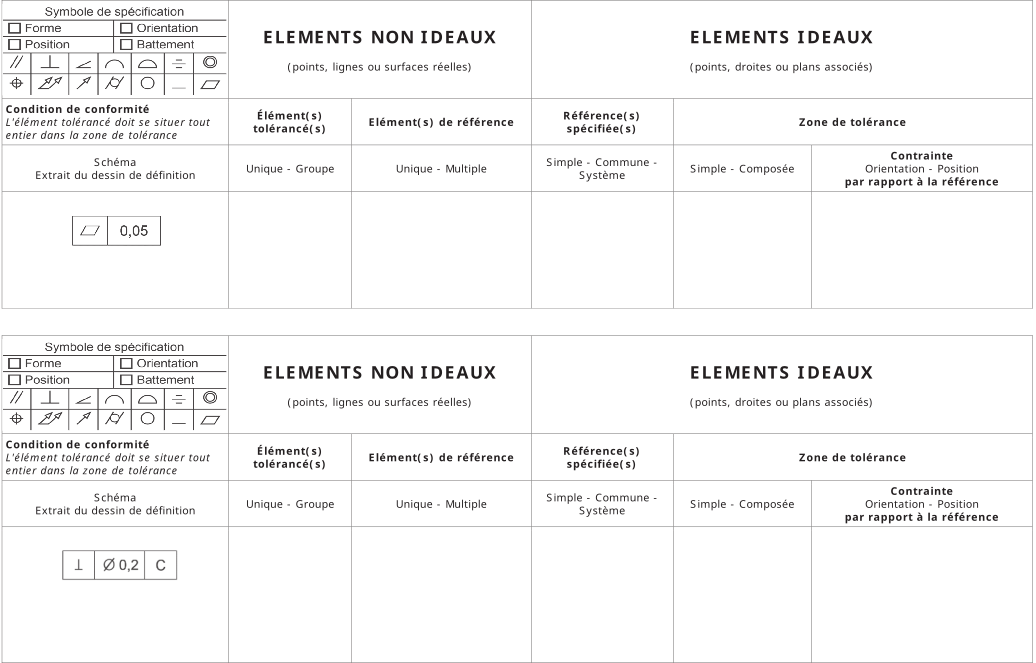
\includegraphics[width=1.35\linewidth,angle=90]{img/DR08.png}
\end{center}}{\begin{center}
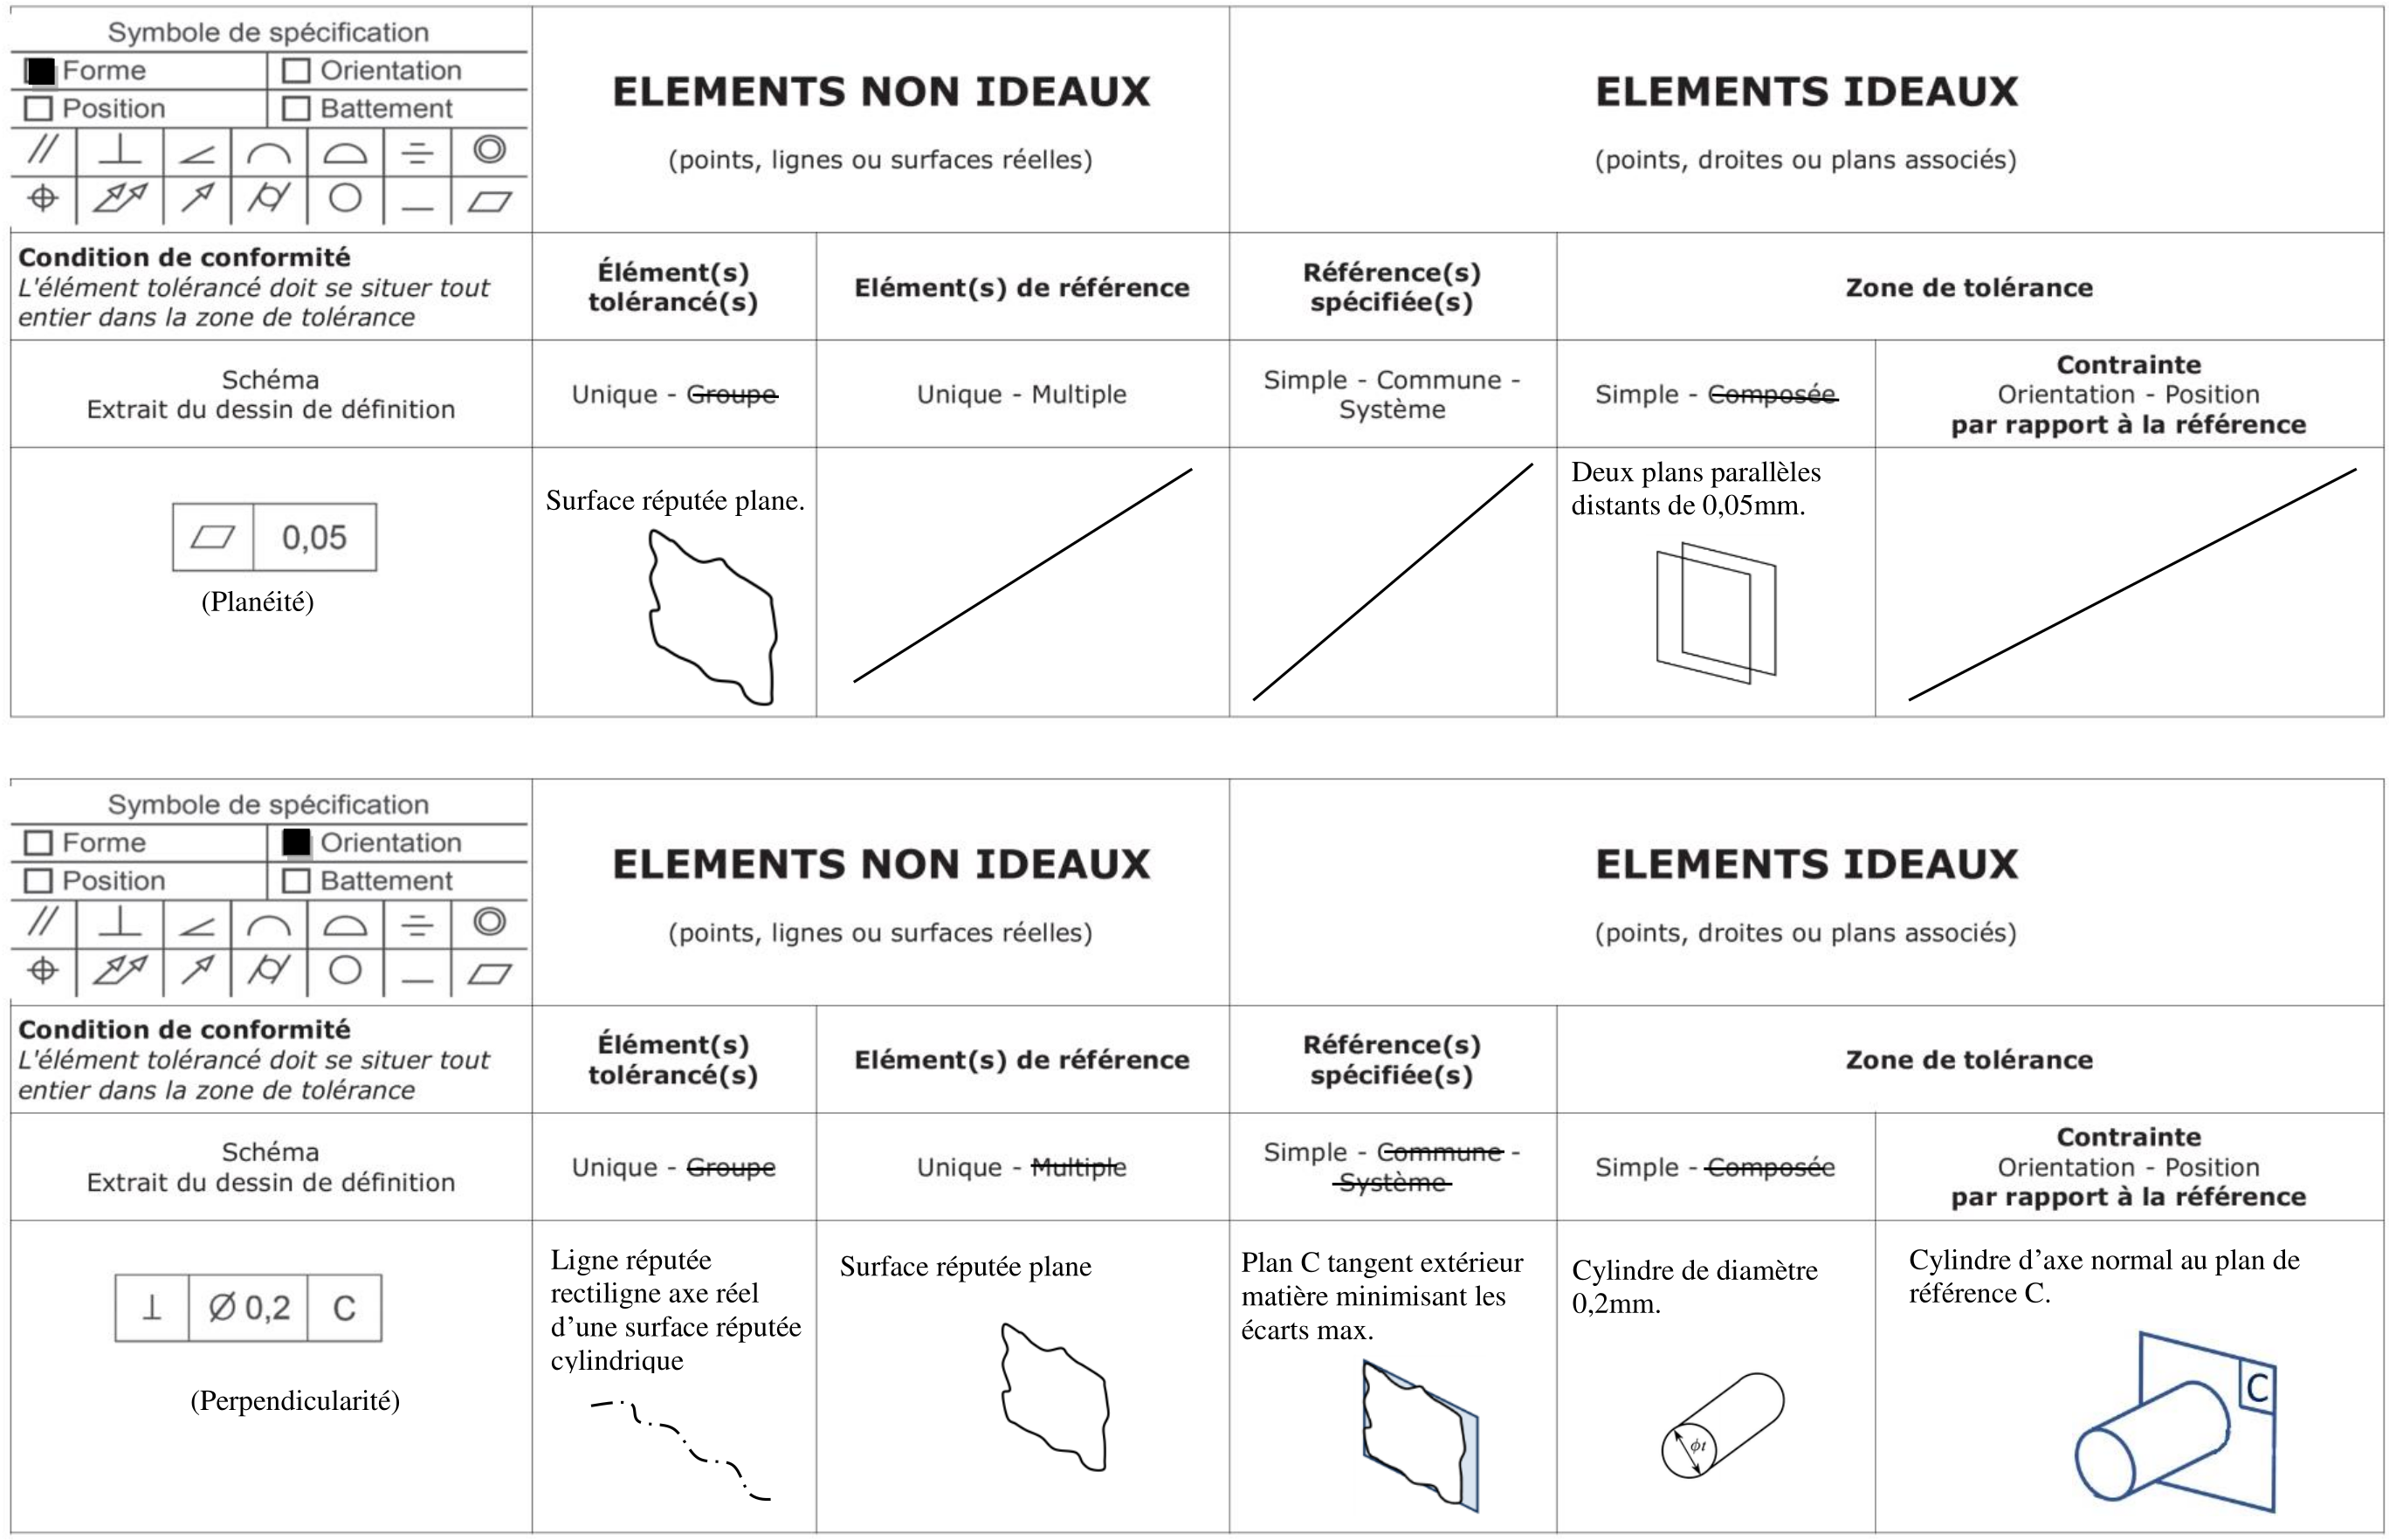
\includegraphics[width=1.35\linewidth,angle=90]{img/DR08_cor.png}
\end{center}}

\reponse{0}{\begin{center}
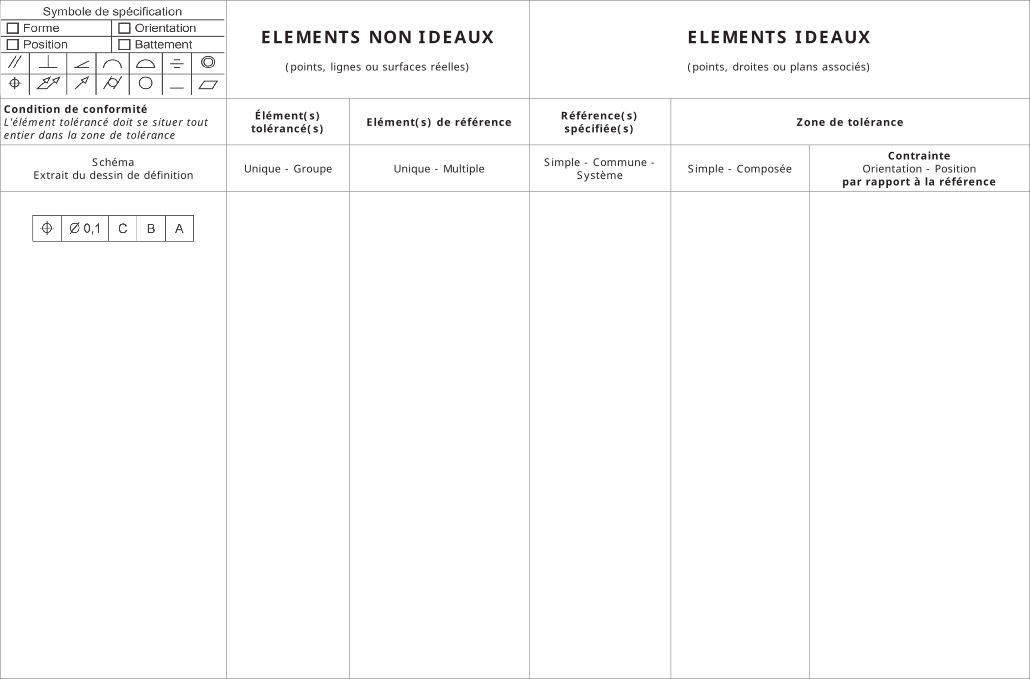
\includegraphics[width=1.35\linewidth,angle=90]{img/DR09.png}
\end{center}}{\begin{center}
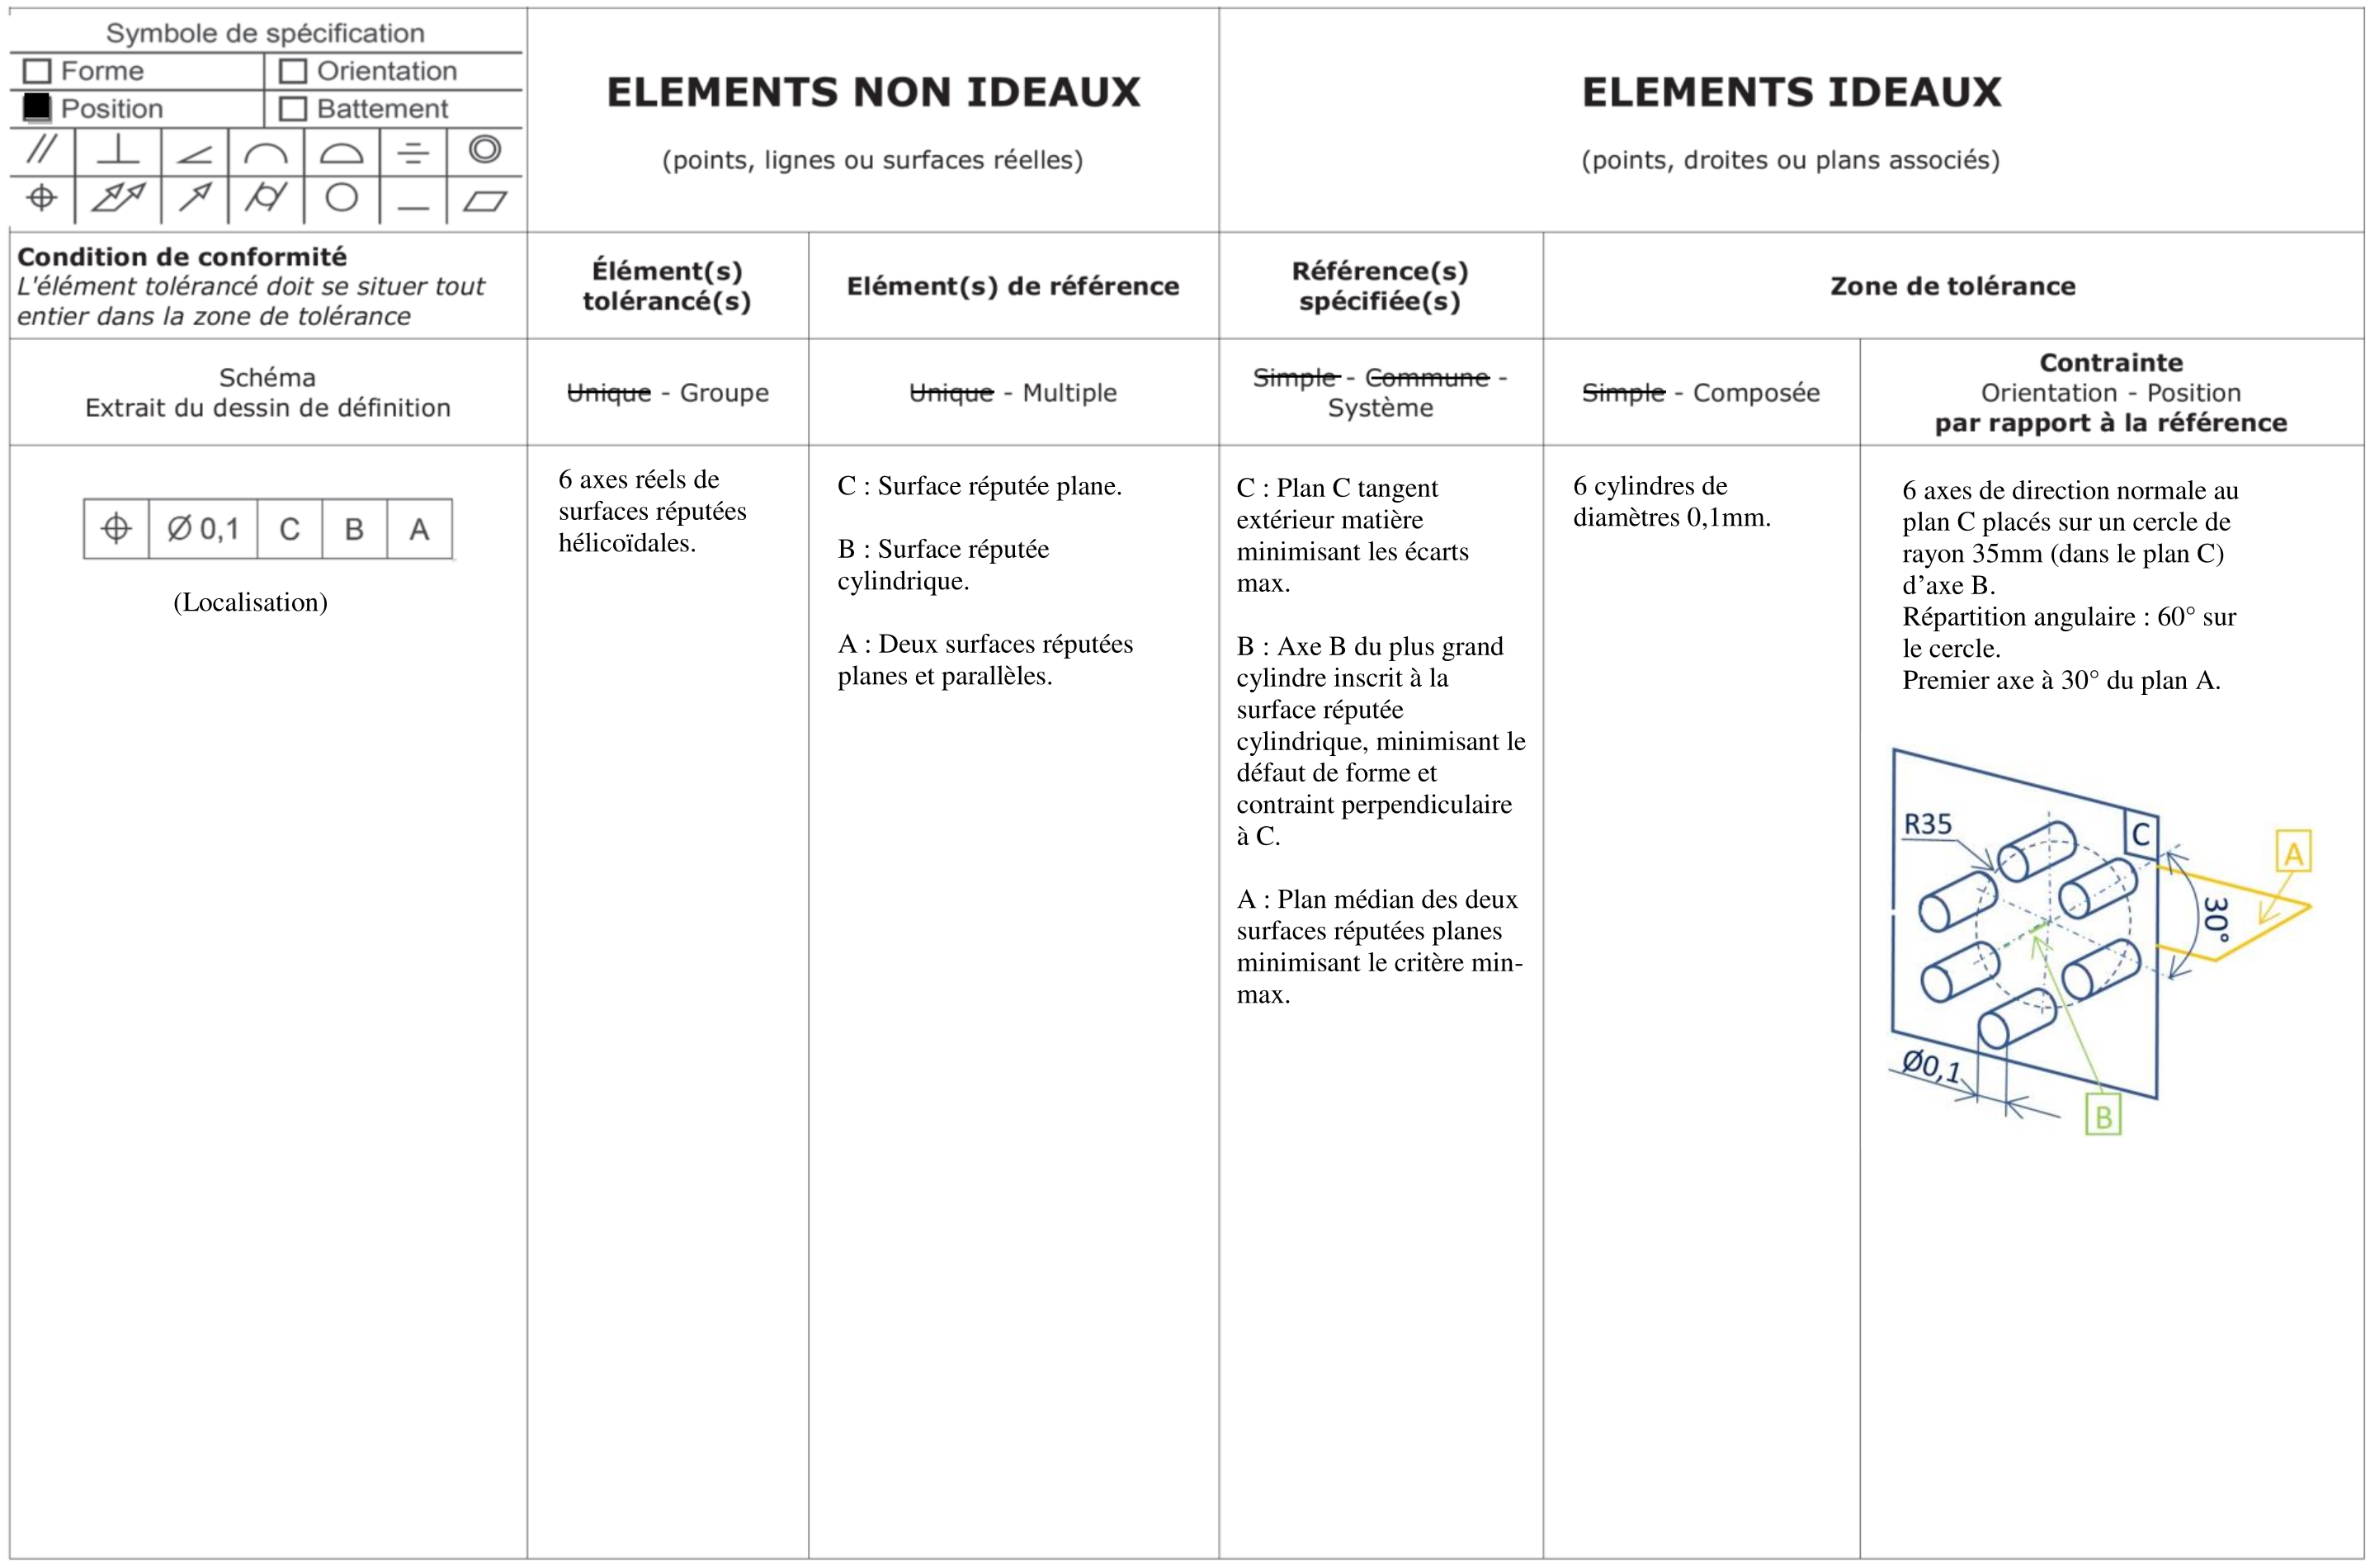
\includegraphics[width=1.35\linewidth,angle=90]{img/DR09_cor.png}
\end{center}}

\end{document}

